% template file include
\input{template}
\usepackage{tikz}
\usetikzlibrary{shapes.geometric, arrows.meta, positioning, shadows}

% lstlisting stílus
\lstset{
    inputencoding=utf8,
    extendedchars=true,
    basicstyle=\small\ttfamily,
    breaklines=true,
    frame=single,
    captionpos=b,
    numbers=left,
    numberstyle=\tiny,
    numbersep=5pt,
    tabsize=4,
    showstringspaces=false,
    literate=
        {á}{{\'a}}1 {é}{{\'e}}1 {í}{{\'i}}1 {ó}{{\'o}}1 {ö}{{\"o}}1
        {ő}{{\H o}}1 {ú}{{\'u}}1 {ü}{{\"u}}1 {ű}{{\H u}}1
        {Á}{{\'A}}1 {É}{{\'E}}1 {Í}{{\'I}}1 {Ó}{{\'O}}1 {Ö}{{\"O}}1
        {Ő}{{\H O}}1 {Ú}{{\'U}}1 {Ü}{{\"U}}1 {Ű}{{\H U}}1
}


% =========================================
% Rövidítések automatikus kezelése
% =========================================
\usepackage[acronym,automake]{glossaries-extra}
\makeglossaries

% Rövidítések stílusa:
\setabbreviationstyle[acronym]{long-short}

\usepackage[utf8]{inputenc}



\begin{document}
 

\pagenumbering{gobble}

% ELŐLAPOK: borító, feladatlap, nyilatkozat, konzultációs napló
% Gyors szerkesztéshez kommentezd ki az alábbi 4 sort — kb. 40%-kal gyorsítja a fordítást
 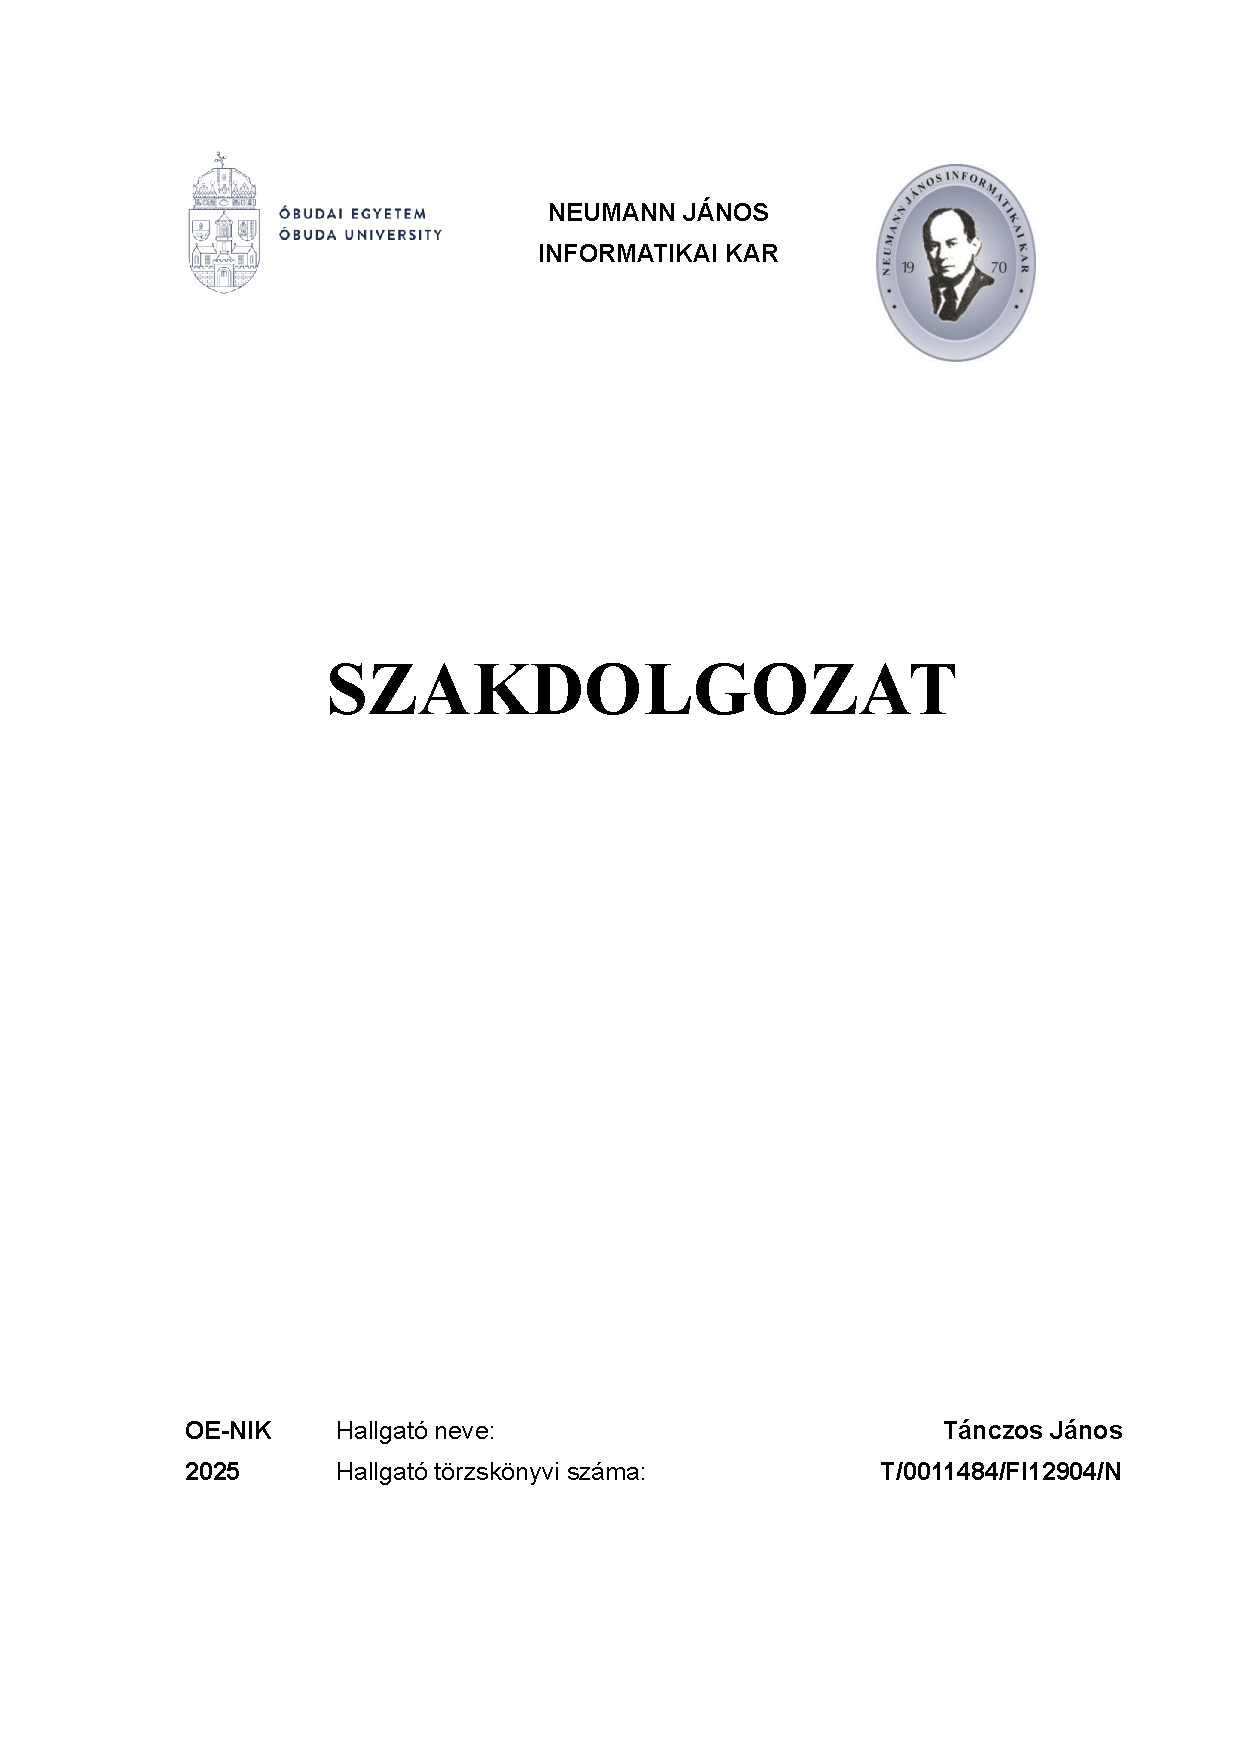
\includepdf[pages=-]{includes/BELSO-BORITOLAP_DM.pdf}
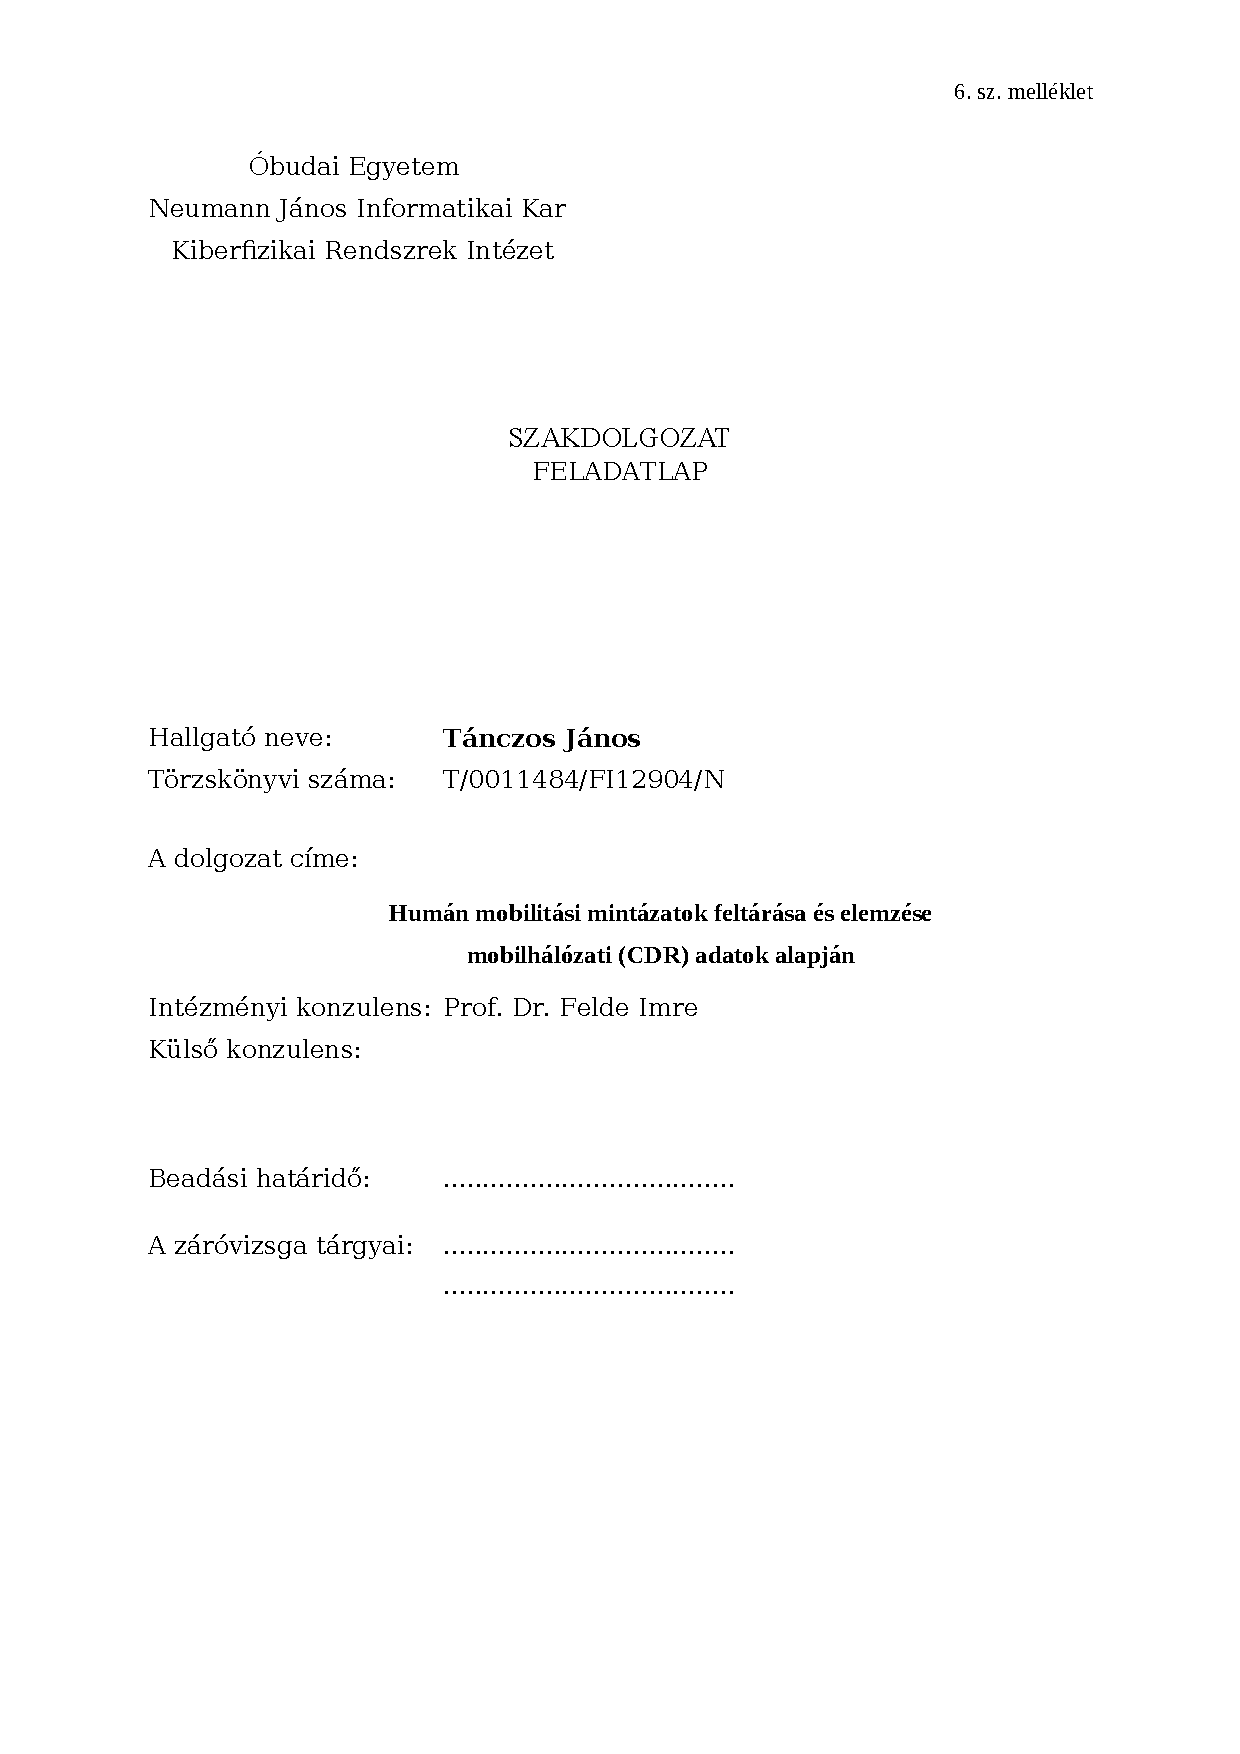
\includepdf[pages=-]{includes/FELADATLAP.pdf}

\includepdf[pages=-]{includes/HALLGATOI-NYILATKOZAT_DM.pdf}
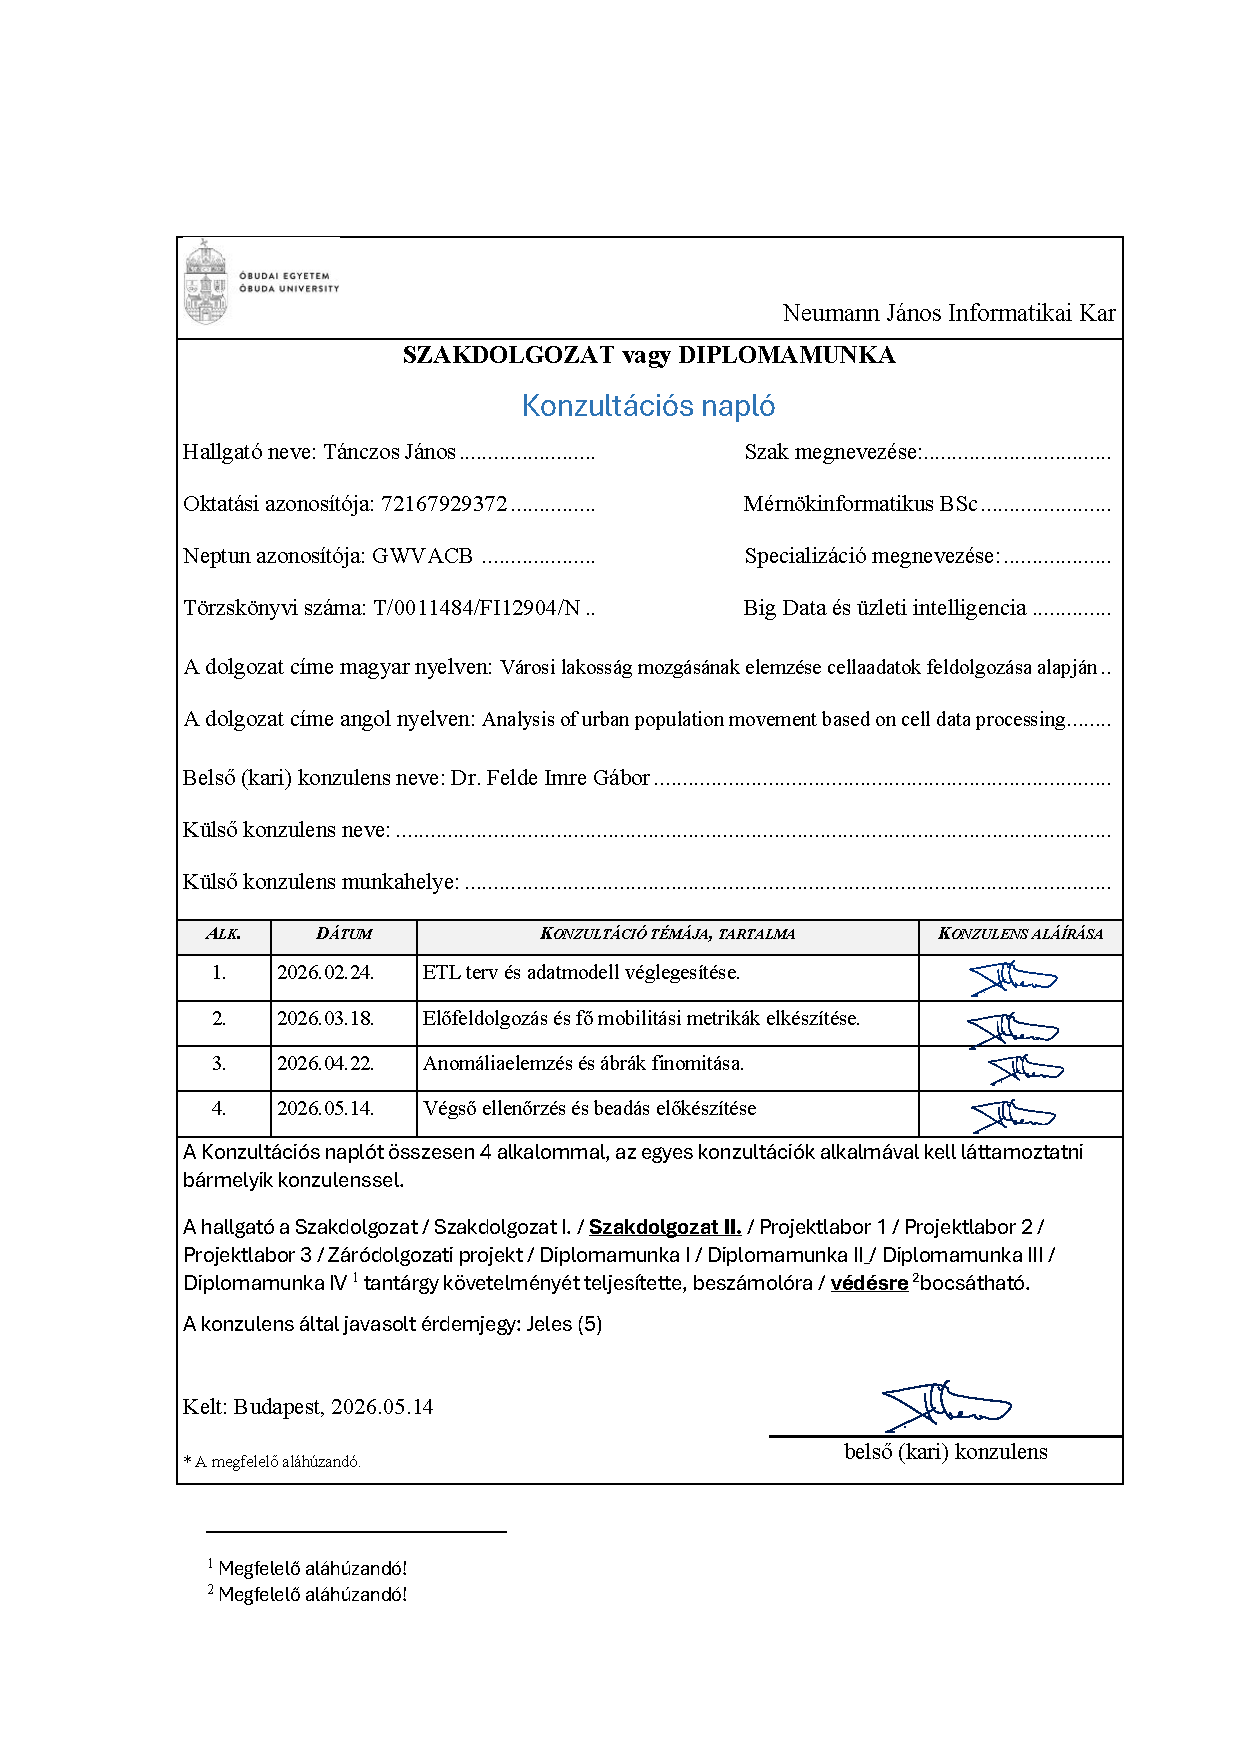
\includepdf[pages=-]{includes/KONZULTACIOS-NAPLO_DM2_NAPPALI.pdf}




\section*{ABSZTRAKT}

A mobiltelefon-hálózatok működése során keletkező cellaforgalmi adatok (\textit{Call Detail Records} – CDR) az emberi mozgás nagy felbontású, passzív nyomon követésére alkalmas adatforrást jelentenek. E dolgozat célja egy nyílt forráskódú CDR adathalmaz feldolgozására képes rendszer megtervezése és megvalósítása, a belőle kinyerhető mobilitási metrikák kiszámítása, valamint az eredmények térinformatikai megjelenítése.

A munka az YJMob100K adatkészleten alapul, amely Nagoya városából (Japán) 100\,000 felhasználó 75 napos, 30 perces felbontású mozgásadatát tartalmazza – összesen közel 141 millió rekordot. Az ETL-folyamat DuckDB oszlopos adatbázis-kezelőre épül; felhasználónként és naponként kerül kiszámításra a gyrációs sugár (\textit{radius of gyration}), a Shannon-entrópia, a helydiverzitás, valamint az otthon–munkahely távolság. A térbeli vizualizáció GeoPandas és pyproj könyvtárakkal, EPSG:2449–WGS84 georeferálással, OpenStreetMap alaptérkép felett készült. A rendellenes mozgásminták azonosítása Isolation Forest algoritmussal történt.

Az eredmények szerint a felhasználók napi mozgásterének mediánja 3\,435~méter, az otthon–munkahely távolság mediánja 3\,589~méter; a felhasználók 27,8 százaléka napi 10~km-nél messzebbre ingázik. A vészhelyzeti időszakban azonosított rendellenes felhasználók gyrációs sugara 4,52-szere, otthon–munkahely távolsága közel 11-szerese a normális értékeknek.

\vspace{0.5em}
\noindent\textbf{Kulcsszavak:} CDR, mobilhálózat, emberi mobilitás, gyrációs sugár, DuckDB, anomáliadetekció, GIS, YJMob100K

\newpage
\section*{ABSTRACT}

Call Detail Records (CDR) generated by mobile phone networks provide a high-resolution, passively collected source for tracking human mobility. This thesis presents the design and implementation of a pipeline for processing an open-source CDR dataset, computing mobility metrics, and visualising the results using geographic information system (GIS) tools.

The work is based on the YJMob100K dataset, which captures the movement of 100,000 anonymous users over 75 days at 30-minute intervals in Nagoya, Japan, comprising approximately 141 million records. The ETL pipeline is built on DuckDB, a columnar in-process database engine; computed metrics include the radius of gyration, Shannon entropy, location diversity, and home–workplace distance, calculated per user and per day. Spatial visualisation was performed using GeoPandas and pyproj with reprojection from EPSG:2449 to WGS84, overlaid on OpenStreetMap basemaps. Anomalous mobility patterns were detected using the Isolation Forest algorithm.

Results show a median daily radius of gyration of 3,435~m and a median home–workplace distance of 3,589~m, with 27.8\% of users commuting more than 10~km per day. During the emergency period, anomalous users exhibited a radius of gyration 4.52 times larger and a home–workplace distance nearly 11 times greater than non-anomalous users.

\vspace{0.5em}
\noindent\textbf{Keywords:} CDR, mobile network, human mobility, radius of gyration, DuckDB, anomaly detection, GIS, YJMob100K



% TARTALOMJEGYZÉK
\newpage
\pagenumbering{arabic}
\tableofcontents
\newpage


% -----------------------------------------------------

% ITT KELL HOZZÁADNI A FEJEZETEKET, CÍM NAGYBETŰVEL:

\clearpage
\section{BEVEZETÉS}
% !TEX root = ../main.tex
\subsection{Motiváció}

Az okostelefonok mindennapjaink részévé válásával a mobilhálózatban keletkező cellainformációk -- viselkedési mintázatokat, útvonalakat és szokásokat rajzolnak ki rólunk.

\enquote{\textit{The continuous communication between a device and the Mobile Phone Network leaves traces… the Mobile Phone Network can ‘sense’ our movements.}}%
\cite{pinter2021evaluating}

A Call Detail Record (CDR) látszólag egyszerű adatforrás: időbélyegek, cellaváltások, aktivitások. Mégis alkalmas az emberi mobilitás szabályszerűségeinek feltárására, így értékes alap a várostervezés, a közlekedési analitika és a viselkedéskutatás számára.

%\begin{figure}[H]
 %   \centering
  %  
\includegraphics[width=0.70\textwidth]{img/BigDataFigure.jpg}
   % \caption{A „Big Data” fogalom vizuális megjelenítése. }
    %\label{fig:celltower_flickr}
    %\vspace{0.2cm}
%\end{figure}

%\subsection{A probléma}

%A modern városok működése összetett, sűrű és sokszínű rendszer, amelyben az emberek mindennapi mozgásai alapvetően meghatározzák az infrastruktúra terhelését, a szolgáltatások igénybevételét és a közlekedési hálózat dinamikáját. Mégis: a legtöbb esetben a városi mobilitás megértése ma is csak részleges, megfigyelésekre, kérdőívekre vagy különálló mérési pontokra épül.

%A CDR-adatok lehetőséget adnak egy sokkal részletesebb képre: arra, hogy embertömegek kollektív viselkedését vizsgáljam, anélkül, hogy az egyén privát szférája sérülne. Ez az adat azonban csak nyers forma értelmezés, feldolgozás és modellezés nélkül nem nyújt közvetlenül információt.


%A feladat ráadásul nem csupán matematikai vagy algoritmikus jellegű. A mobilitási jellemzők mint a radius of gyration, az útvonalak (trajectory), vagy épp az entropy-alapú mutatók társadalmi, gazdasági és urbanisztikai következtetések alapjai lehetnek. E paraméterek kiszámítása tehát érzékeny, ugyanakkor nagy értékű információ.

\subsection{A dolgozat célkitűzései}
\label{subsec:goals}

A dolgozat célja egy olyan rendszer megtervezése és teljes körű implementálása, amely egy nyílt forráskódú CDR-adathalmazon felhasználói szintű mobilitási mintázatokat tár fel és térinformatikai eszközökkel jelenít meg. Részcélok:

\begin{enumerate}
    \item \textbf{Szakirodalmi megalapozás.} A CDR-feldolgozás bevett megoldásai és a mobilitási metrikák (\textit{Radius of Gyration}, entrópia, \textit{trajectory}) számítása.
    \item \textbf{Adatkészlet bemutatása.} Az YJMob100K szerkezete, a baseline és a vészhelyzeti részkészletek viszonya, POI-fájlok.
    \item \textbf{Rendszerterv.} 16~GB~RAM-os egygépes környezetben is hatékony architektúra 141~M rekordhoz.
    \item \textbf{ETL-pipeline.} Adatbetöltéstől a felhasználónkénti, naponkénti metrikák számításáig, csillagsémás tárolással.
    \item \textbf{Anomáliadetekció.} Felügyelet nélküli azonosítás, baseline-visszaösszevetéssel.
    \item \textbf{GIS-megjelenítés.} Rácskoordináták georeferálása és OSM-alapú megjelenítés.
    \item \textbf{Két pilléres kiértékelés.} \textbf{(A)} egyéni városhasználat (K-Means archetípusok, POI-affinitás, helyszín-azonosított rendezvények) és \textbf{(B)} kollektív vészhelyzeti viselkedés (Isolation Forest paradoxon, ,,ébredő város'', esemény-elnémulás) -- a CDR-szakirodalom (González \cite{gonzalez2008understanding}, Pintér--Felde \cite{pinter2021evaluating, pinter2022awakening}, Traag et al.\ \cite{traag2011social}) megfigyeléseivel kvantitatívan összevetve.
\end{enumerate}

\subsection{A dolgozat felépítése}
\label{subsec:structure}

A 2--4.\ fejezet az elméleti hátteret adja: a CDR fogalma és a mobilhálózati architektúra (2), a CDR-alapú mobilitáskutatás és smart~city alkalmazások szakirodalmi áttekintése (3), valamint a mobilitási metrikák matematikai definíciói (4). Az 5.\ fejezet az YJMob100K adathalmazt mutatja be. A 6--8.\ fejezet a megvalósítást tárgyalja: rendszerterv és csillagséma (6), implementáció SQL-kódmintákkal (7), georeferálás és tematikus GIS-térképek (8). A 9.\ fejezet a két pillér (egyéni profilok / vészhelyzeti kollektív viselkedés) kvantitatív elemzéseit, a 10.\ fejezet az összefoglalást és a jövőbeli irányokat tartalmazza. A POI-zóna leképezés a Függelékben található.


\clearpage
\section{ELMÉLETI HÁTTÉR: MOBILHÁLÓZATOK ÉS CDR}
% !TEX root = ../main.tex
\subsection{Mobiltelefon-hálózatok felépítése röviden}
A mobiltelefon-hálózatok cellás architektúrán alapulnak. Egy szolgáltató területét kisebb cellákra osztja, melyek közepén bázisállomások (torony, antenna) helyezkednek el. Egy készülék mindig a legközelebbi toronyhoz csatlakozik, és a hálózat szükség esetén cellaváltást hajt végre. A mobilitás során úgynevezett „handover” folyamaton megy keresztül, amikor a hálózat áthelyezi az eszközt egy másik cellára. Az adatok pontosságát a cellák mérete határozza meg, városi környezetben a sűrűn telepített tornyok miatt az ellátási terület akár 2~km$^{2}$ alatti is lehet, míg vidéken a cellák több négyzetkilométert fednek le \cite{gonzalez2008understanding, pinter2022awakening}. A mobiltoronyok nagy lefedettsége miatt a pozícióbecslés jelentősen durvább a GPS koordinátákhoz képest \cite{gonzalez2008understanding}. Egy rekord csak a kiszolgáló torony azonosítóját tárolja; a cella belső szerkezetéről nem tartalmaz információt \cite{gonzalez2008understanding}.

\begin{figure}[h!]
    \centering
    % A szögletes zárójelben állíthatod a méretet (itt a szövegszélesség 90%-a)
    % A kapcsos zárójelbe írd a lementett kép pontos nevét kiterjesztéssel együtt!
    \includegraphics[width=0.9\textwidth]{img/handover_schema.png}
    
    % Ez jelenik meg a kép alatt:
    \caption{Sematikus cella-architektúra és a cellaváltás (Handover) folyamata}
    
    % Ezzel tudsz hivatkozni rá a szövegben (pl. \ref{fig:handover}):
    \label{fig:handover}
\end{figure} 

\subsection{Call Detail Record fogalma}
A CDR adatok eredetileg számlázási célból létrehozott naplófájl, amely a hálózatban történt aktív eseményeket tartalmazza, mint például a hívásokat, SMS-küldést és mobilinternet-használatot.\cite{pinter2020artificial, zhang2019connected}. 
Az adatkészletekben egy rekord jellemző tartalma:
\begin{itemize}
    \item \textbf{Időbélyeg (Timestamp):} Az esemény pontos dátuma és kezdő időpontja. (Gyakran csonkítják pl. 10 másodperces pontosságra)
    \item \textbf{Anonimizált előfizetői azonosító (Hashed User ID):} Egy pszeudonim, titkosított kulcs, amely az egyedi SIM-kártyát azonosítja.
    \item \textbf{Cella azonosító (Cell ID):} A tranzakciót kiszolgáló bázisállomás egyedi azonosítója.
    \item \textbf{Esemény típusa:} Mobiladat / Hívás / SMS 
    \item \textbf{Eszközinformáció (Opcionális):} Egyes adatkészletek tartalmaznak a TAC (Type Allocation Code) kódot.
\end{itemize}\cite{pinter2022awakening, pinter2020artificial}

Technikai vagy adatvédelmi okokból a kutatói adatkészletek általában nem tartalmazzák az alábbiakat:
\begin{itemize}
    \item \textbf{Passzív cellaváltás (Handover):} Bár a hálózat rögzítheti a cellaváltást, kutatási célokra nem elérhetők \cite{pinter2022awakening}.
    \item \textbf{Pontos pozíció:} A CDR pontossága elmarad a GPS-étől: a sűrűn lakott területeken néhány száz méter, míg vidéken több kilométer is lehet \cite{gonzalez2008understanding}.
    \item \textbf{Szemantikai tartalom:} Kizárólag a metaadatokra (hol, mikor, ki) korlátozódnak; a tartalomra (mit, miért) vonatkozó információ nem áll rendelkezésre \cite{batty2012smart}.
\end{itemize}


\subsection{Adatvédelem és anonimizálás}
Az adatok személyes jellegűek, hiszen a felhasználók mozgását és viselkedési mintáit tartalmazzák. A szolgáltatók ezért az adatokat anonimizálják: az előfizetői azonosítót pszeudoazonosítóval (hashed value) helyettesítik, és elválasztják a számlázási adatbázistól \cite{pinter2022awakening}. A személyazonosítás vagy pontos címek visszakövetése tilos \cite{zhang2019connected}. A Data4Refugees projektnek például a Türk Telekom olyan CDR adatokat bocsátott kutatók rendelkezésére, amelyekben csupán a felhasználó állampolgárságára (török vagy szír) és a hívások irányára vonatkozó információ maradt meg \cite{rhoads2020measuring}. 




\clearpage
\section{SZAKIRODALMI ÁTTEKINTÉS A CDR FELDOLGOZÁSÁRÓL}
% !TEX root = ../main.tex
\subsection{CDR alapú humán mobilitás kutatások}
Az elmúlt húsz évben sok kutató vizsgálta már, hogyan írható le az emberi mozgás CDR adatokkal. Gonzalez és munkatársai például százezer anonim felhasználó adatait elemezték fél évig. Azt találták, hogy az emberek mozgása meglepően szabályos: mindenki leginkább néhány kedvenc helyét keresi fel, és csak ritkán utazik messzire.  
A szerzők a trajektóriák elemzéséhez bevezették a \emph{gyrációs sugár} fogalmát, amely meg mutatja, mekkora területet jár be jellemzően egy alany. Az eloszlása nem egyenletes, hanem vágott hatványfüggvényt követ . Vagyis az emberek mozgása korlátozott, nem járnak be végtelen távolságokat, ritkán tesznek meg nagyobb utakat. Emiatt a bankjegyek mozgásából következtetett Lévy-járás modell nem ragadja meg pontosan, hogyan mozognak ténylegesen az emberek \cite{gonzalez2008understanding}.

Pintér és munkatársai például Budapest CDR-adatait vetették össze az ingatlanárakkal, és világosan látszott: akik rosszabb anyagi helyzetben élnek, azoknak messzebbre kell járniuk dolgozni. A középosztálybeliek ezzel szemben kevesebbet ingáznak, míg a legszegényebb és leggazdagabb csoportoknál nagyobb a napi mozgástávolság. Érdekes módon, ha azt nézték, mennyire sokszínű helyekre járnak az emberek, azaz mekkora az \emph{entrópia}, ott nem találtak erős kapcsolatot a vagyoni helyzettel \cite{pinter2021evaluating}.

Nem csak magyar adatokból vontak le ilyen következtetéseket. Szingapúrban a tehetősebb mobil-előfizetők inkább rövidebb távokat utaznak, Bostonban viszont pont a gazdagabbak járnak távolabbra \cite{pinter2021evaluating}.

A társadalmi szegregáció is mérhető. A szír menekültek és a török lakosság kommunikációs mintái elemzéséből, azt mutatták, hogy a szegregáció jelentősen csökkenthető, ha a lakóhelyi keveredést elősegítjük például célzott lakbértámogatásokkal \cite{rhoads2020measuring}.


\subsection{CDR alkalmazása smart city / urban sensing területeken}

A smart city lényege, hogy az egész városban infokommunikációs technológiák (ICT) működnek, szenzorok figyelnek mindent, és ezek az eszközök folyamatosan, valós időben gyűjtik az adatokat. Rögzítik, mi történik a közlekedésben, hogyan változik az energiafogyasztás, merre mozognak az emberek, és milyen állapotban van az infrastruktúra. Ez a sok érzékelő és adatforrás együtt egyfajta városi „idegrendszert” alkot. Így a város könnyebben optimalizálja a szolgáltatásait, és jobban eléri a fenntarthatósági célokat is.
\cite{batty2012smart}.  % Smart city definíció

Ebben a rendszerben a CDR adatok különösen értékesek. Egyszerűen azért, mert ezek az adatok pontosan megmutatják, mikor és hol vannak a városlakók, hogyan mozognak, ráadásul nagy mennyiségben, folyamatosan és viszonylag olcsón lehet előállítani őket. A CDR-alapú urban sensing alkalmazásokról, több fontos területet is meg kell említeni:

\begin{itemize}
  \item \textbf{Közlekedési igények becslése és forgalmi tervezés.}
A mobilitási mintákból tisztán látszanak a csúcsidőszakok, és az, hol torlódik leginkább a forgalom. Ha az adatokat hagyományos háztartási felmérésekkel kombináljuk, részletes, társadalmi szerkezetet kapunk, amit közlekedési mikroszimulációk alapjaként használhatunk \cite{zhang2019connected}. Ezzel a módszerrel a fényderül, hogy hogyan terhelődnek a városi rendszerek, és mennyire képesek alkalmazkodni a változásokhoz.

  \item \textbf{Nagy társadalmi események azonosítása.}
A térben és időben jelentkező anomáliák egyértelműen jelezhetik a tömegrendezvényeket \cite{traag2011social, xavier2012analyzing}. Ezek ismerete nemcsak a várostervezésben, hanem a hálózati terhelés menedzselésében is hasznos lehet.

  \item \textbf{Turizmus és várostervezés támogatása.}
A gyrációs sugár, entrópia és más mobilitási indikátorok térképre vetítve megmutatják, merre mozognak a turisták és a helyiek. Ezek alapján átgondoltabban lehet elhelyezni közszolgáltatásokat, turisztikai attrakciókat vagy új közlekedési kapcsolatokat \cite{pinter2021evaluating, pinter2022awakening}.

  \item \textbf{Digitális epidemiológia és vészhelyzet-kezelés.}
 Járványok vagy más rendkívüli helyzetek idején a mobilitás változásának nyomon követése kulcsfontosságú. A CDR adatokból látható, hogyan reagál a lakosság a korlátozásokra.\cite{pinter2022awakening}. Ezek az információk segítik a döntéshozókat a beavatkozások tervezésében és értékelésében.
\end{itemize}

\subsection{Kutatási célú CDR-adatkészletek általános jellemzői}
\label{subsec:cdr_datasets_general}

A mobilhálózati adatokhoz való hozzáférés jellemzően korlátozott; a szolgáltatók ritkán teszik közzé a teljes adatállományokat. A kutatásokban ezért gyakran anonimizált, kutatási célra dedikált adatkészletekkel dolgoznak \cite{rhoads2020measuring, zhang2019connected}. Egy tipikus adatkészlet egy adott földrajzi régió mobilforgalmát tartalmazza meghatározott időablakban (pl.\ egy hónap vagy év), amely alkalmas a napi és heti trendek vizsgálatára \cite{pinter2022awakening}. A térbeli felbontás javítása érdekében a bázisállomások lefedettségi területét gyakran Voronoi-tesszellációval közelítik (\autoref{fig:voronoi}).

\begin{figure}[ht]
    \centering
    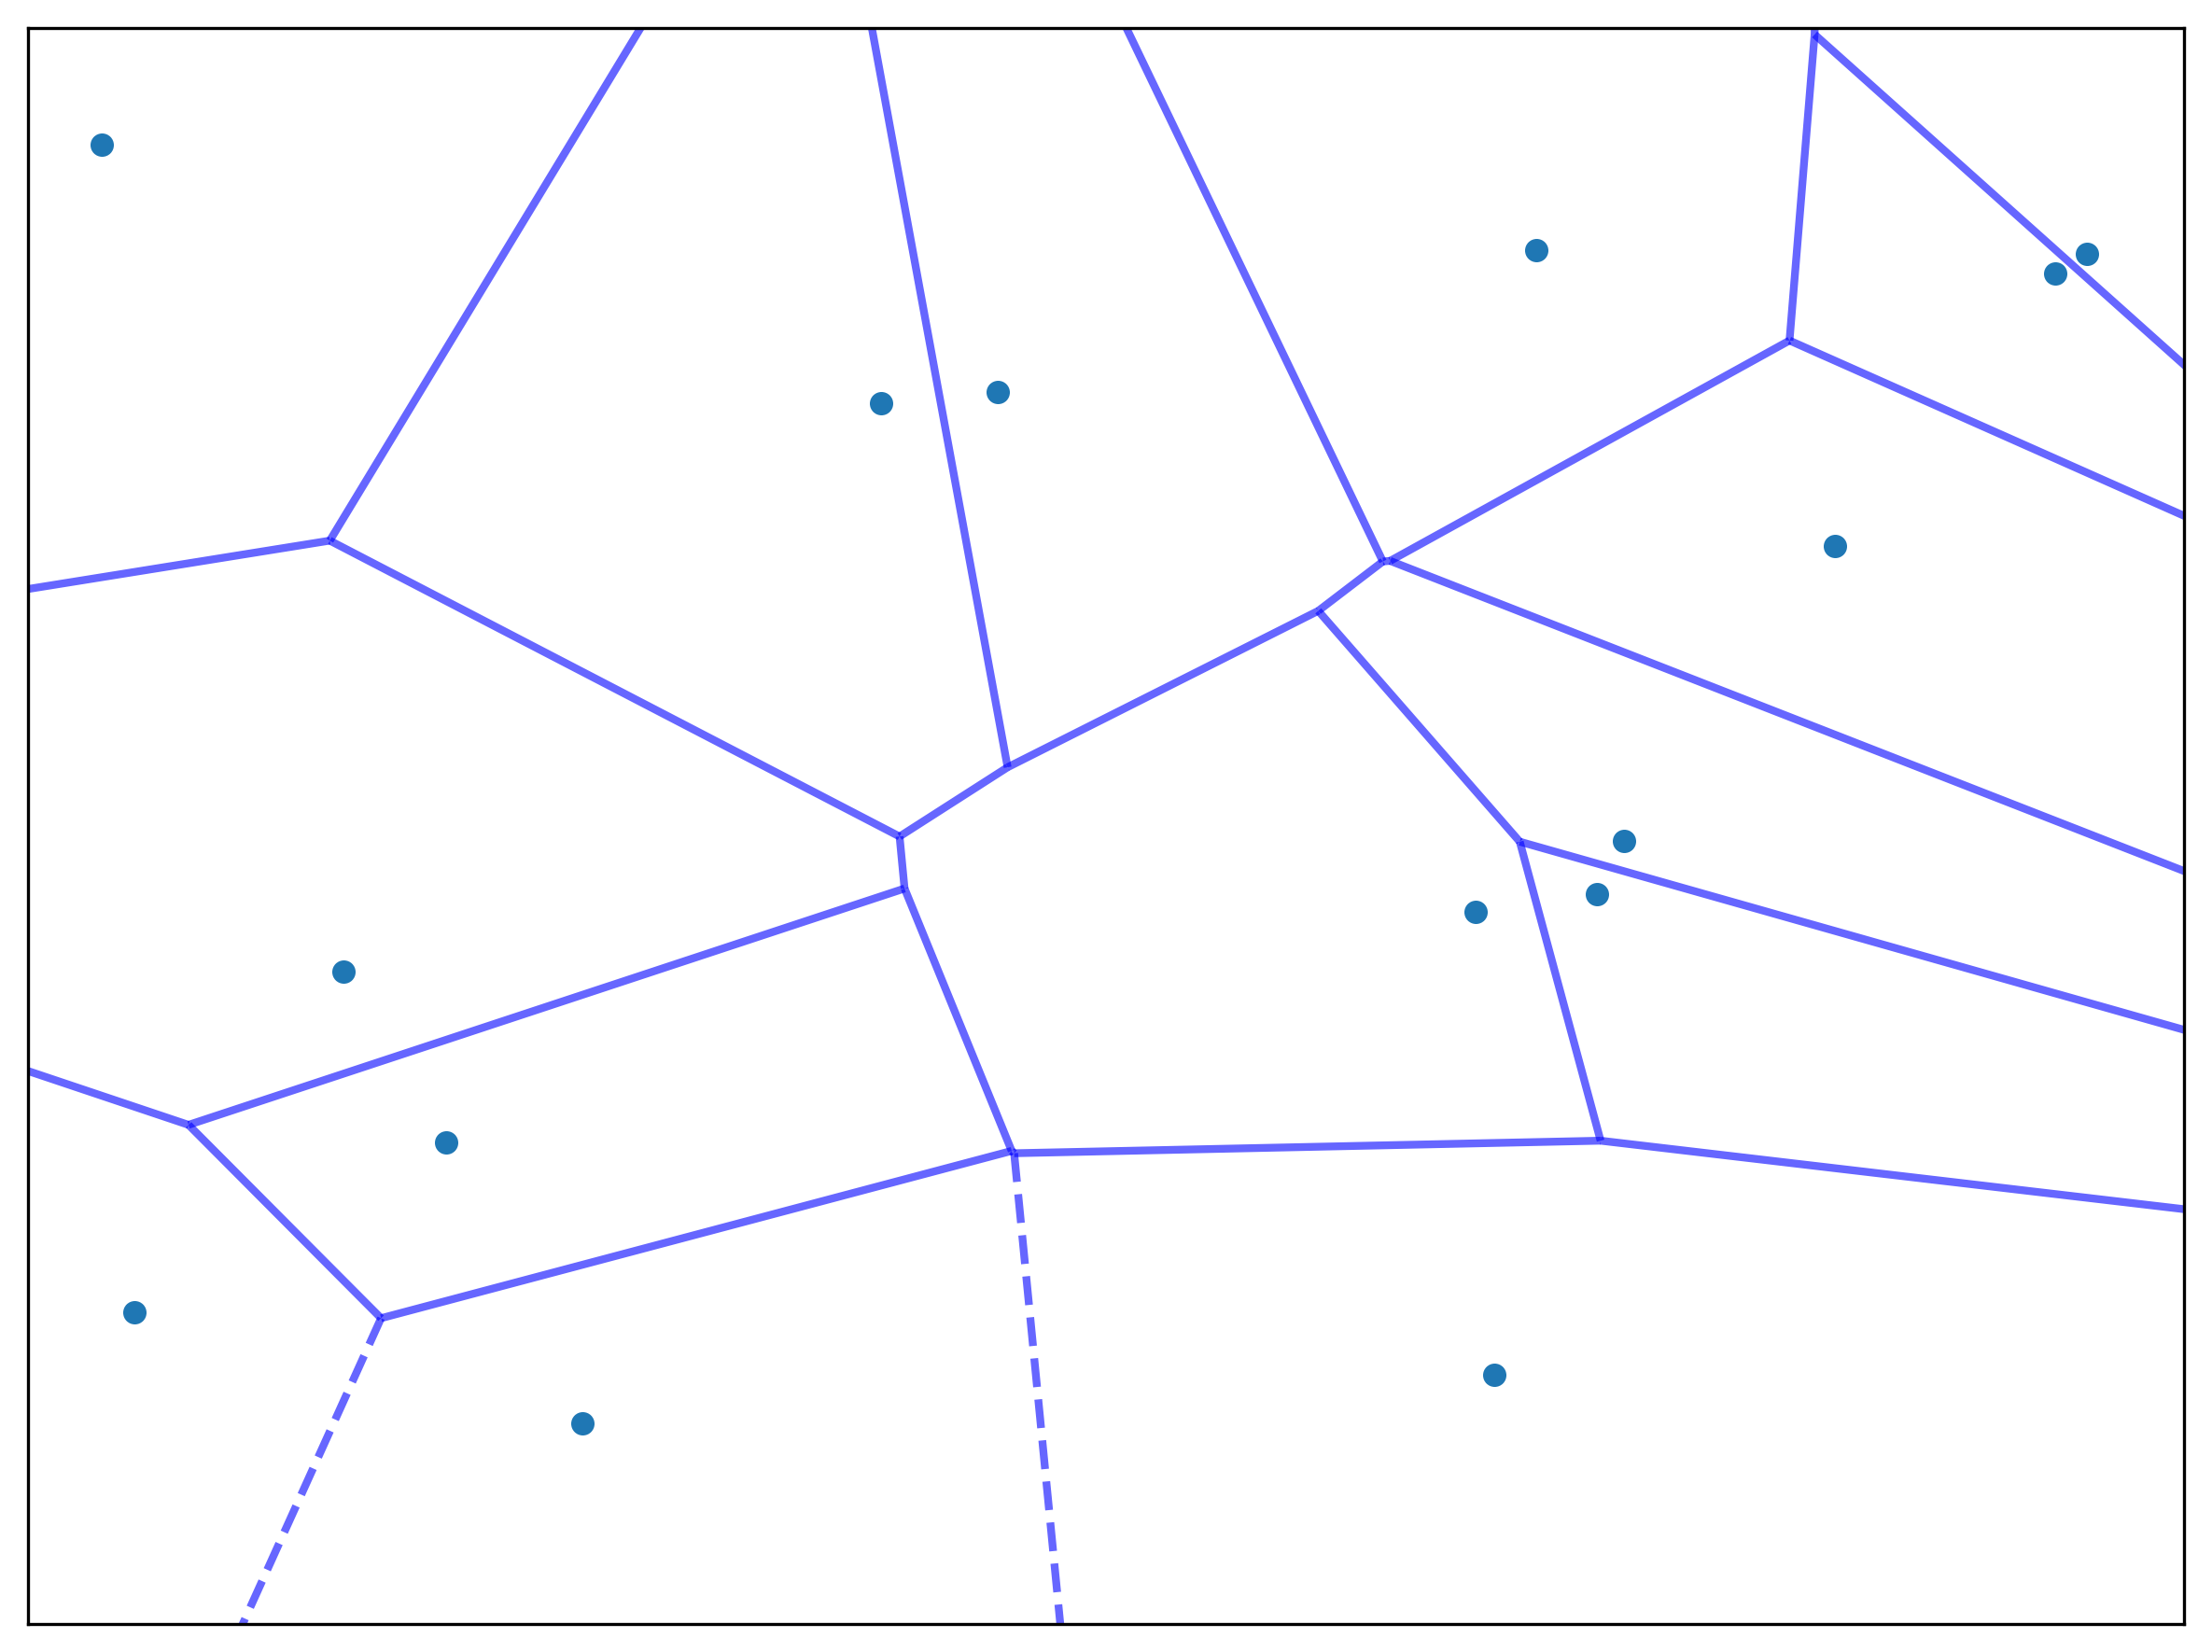
\includegraphics[width=0.4\textwidth]{img/voronoi_example.png}
    \caption{A bázisállomások lefedettségi területének becslésére használt Voronoi-tesszelláció sematikus ábrázolása. A kék pontok a bázisállomásokat, a vonalak a becsült cellahatárokat jelölik.}
    \label{fig:voronoi}
\end{figure}

\subsubsection{Tipikus adatszerkezet és mezők}

A kutatási célú CDR-adatbázisok szerkezete általában relációs modellt használ, amely lehetővé teszi a hatékony elemzést. A következő táblaszerkezet tekinthető általánosnak \cite{pinter2020artificial, pinter2022awakening}:

\begin{itemize}
    \item \textbf{Eseménytábla (CDR Raw):} A tranzakciós tábla, ahol minden sor egy hálózati eseményt ír le. Kulcsmezői: az előfizető pszeudoazonosítója (\textit{Hashed ID}), a cella azonosítója (\textit{Cell ID}), a pontos időbélyeg (\textit{Timestamp}), valamint az esemény típusa (hívás, SMS, adat).

    \item \textbf{Cella metaadatok (Cell Dimension):} A hálózati topológiát leíró tábla, amely tartalmazza a cella azonosítóját és a bázisállomás földrajzi koordinátáit (szélesség, hosszúság). A pontos lefedettségi terület becslésére gyakran Voronoi-tesszellációt alkalmaznak \cite{pinter2020artificial}.

    \item \textbf{Előfizetői attribútumok (Subscriber Dimension):} Az anonim azonosítóhoz kapcsolt statikus adatok. Adatvédelmi okokból ez gyakran korlátozott, de tartalmazhat technikai jellegű információkat, mint például az eszköz típusa (TAC kód alapján) vagy az előfizetés jellege (prepaid/postpaid) \cite{pinter2022awakening}.

    \item \textbf{Származtatott mobilitási metrikák (Derived Features):} Az elemzések során előállított aggregált tábla, amely időszakonként tartalmazza a felhasználókra számított mutatókat (pl.\ gyrációs sugár, entrópia, otthon/munkahely becsült helye) \cite{pinter2021evaluating}.
\end{itemize}

Az adatok térbeli elemzését gyakran segíti egy kiegészítő állomány, amely a cellákat közigazgatási egységekhez (pl.\ kerületek) vagy egységes rácshálóhoz rendeli \cite{rhoads2020measuring}. A 6.\ fejezetben bemutatott rendszerterv ezt az általános modellt adaptálja az YJMob100K rácsalapú szerkezetére.

\subsubsection{Adatminőség, korlátok és etikai keretek}

A nyílt vagy harmadik fél által biztosított CDR-állományok elemzésekor több technikai és módszertani korlátot kell figyelembe venni:

\begin{itemize}
    \item \textbf{Reprezentativitás:} Az adatok általában egyetlen szolgáltatótól származnak, így a piaci részesedéstől függően a teljes populáció csak részben reprezentált \cite{pinter2022awakening}.

    \item \textbf{Passzív adatok hiánya:} A kutatói adatkészletek jellemzően csak az aktív (számlázott) eseményeket tartalmazzák, a passzív cellaváltásokat (\textit{handover}) nem. Ez ritkább mintavételezést eredményez, ami megnehezíti a folyamatos mozgáskövetést \cite{pinter2022awakening}.

    \item \textbf{Térbeli felbontás:} A cellák eltérő mérete miatt a sűrűn lakott városi területek mobilitása pontosabban, míg a vidéki területeké durvábban becsülhető \cite{gonzalez2008understanding}.
\end{itemize}

Az egyéni visszakövetés elkerülése érdekében pszeudo-azonosítókat használnak, és a kutatók számára gyakran csak minimális demográfiai adatokat tesznek hozzáférhetővé, ahogy azt a Data4Refugees projekt esetében is láthatjuk \cite{zhang2019connected}.


\clearpage
\section{MOBILITÁSI METRIKÁK SZÁMÍTÁSI ELJÁRÁSAINAK ÁTTEKINTÉSE}
% !TEX root = ../main.tex
\subsection{Trajektóriák és mozgásleírás CDR-ből}
A CDR adatok időrendbe rendezett cellasorozatokként értelmezhetők. Egy előfizető
útvonala $T_{a}=\{(c_{1},t_{1}),(c_{2},t_{2}),\dots,(c_{n},t_{n})\}$, ahol
$c_{i}$ a kiszolgáló cella azonosítója, $t_{i}$ pedig az esemény időpontja. A
cella koordinátái vagy a torony centruma külön adattáblából származnak. A rekonstrukció
során jellemzően \textbf{időintervallum-alapú interpolációt} alkalmaznak. Az események
közötti időszakot ilyenkor a felhasználó \textbf{utolsó ismert cellájához}
rendelik. Emellett számolnak azzal is, hogy a cellaváltások egy része pusztán
\textbf{handover folyamat}, és nem feltétlenül valódi helyváltoztatás
\cite{pinter2022awakening}.

\subsection{Radius of Gyration (gyrációs sugár)}

A gyrációs sugár ($r_{g}$) az egyéni mobilitás hatótávolságának alapvető mérőszáma,
amely a meglátogatott helyek tömegközépponttól való átlagos négyzetes távolságát
fejezi ki \cite{pinter2021evaluating}. Jelölje $N$ a vizsgált időszakban rögzített
események számát, $\vec{r}_{i}$ az $i$-edik esemény helyszínének koordinátáit, $\vec
{r}_{\mathrm{cm}}= \frac{1}{N}\sum_{i=1}^{N}\vec{r}_{i}$ pedig a trajektória tömegközéppontját.
Ekkor a gyrációs sugár definíciója:

\begin{equation}
	r_{g} = \sqrt{\frac{1}{N}\sum_{i=1}^{N}\|\vec{r}_{i} - \vec{r}_{\mathrm{cm}}\|^{2}}
	.
\end{equation}
\begin{figure}[h!]
    \centering
    % A képfájl neve:
    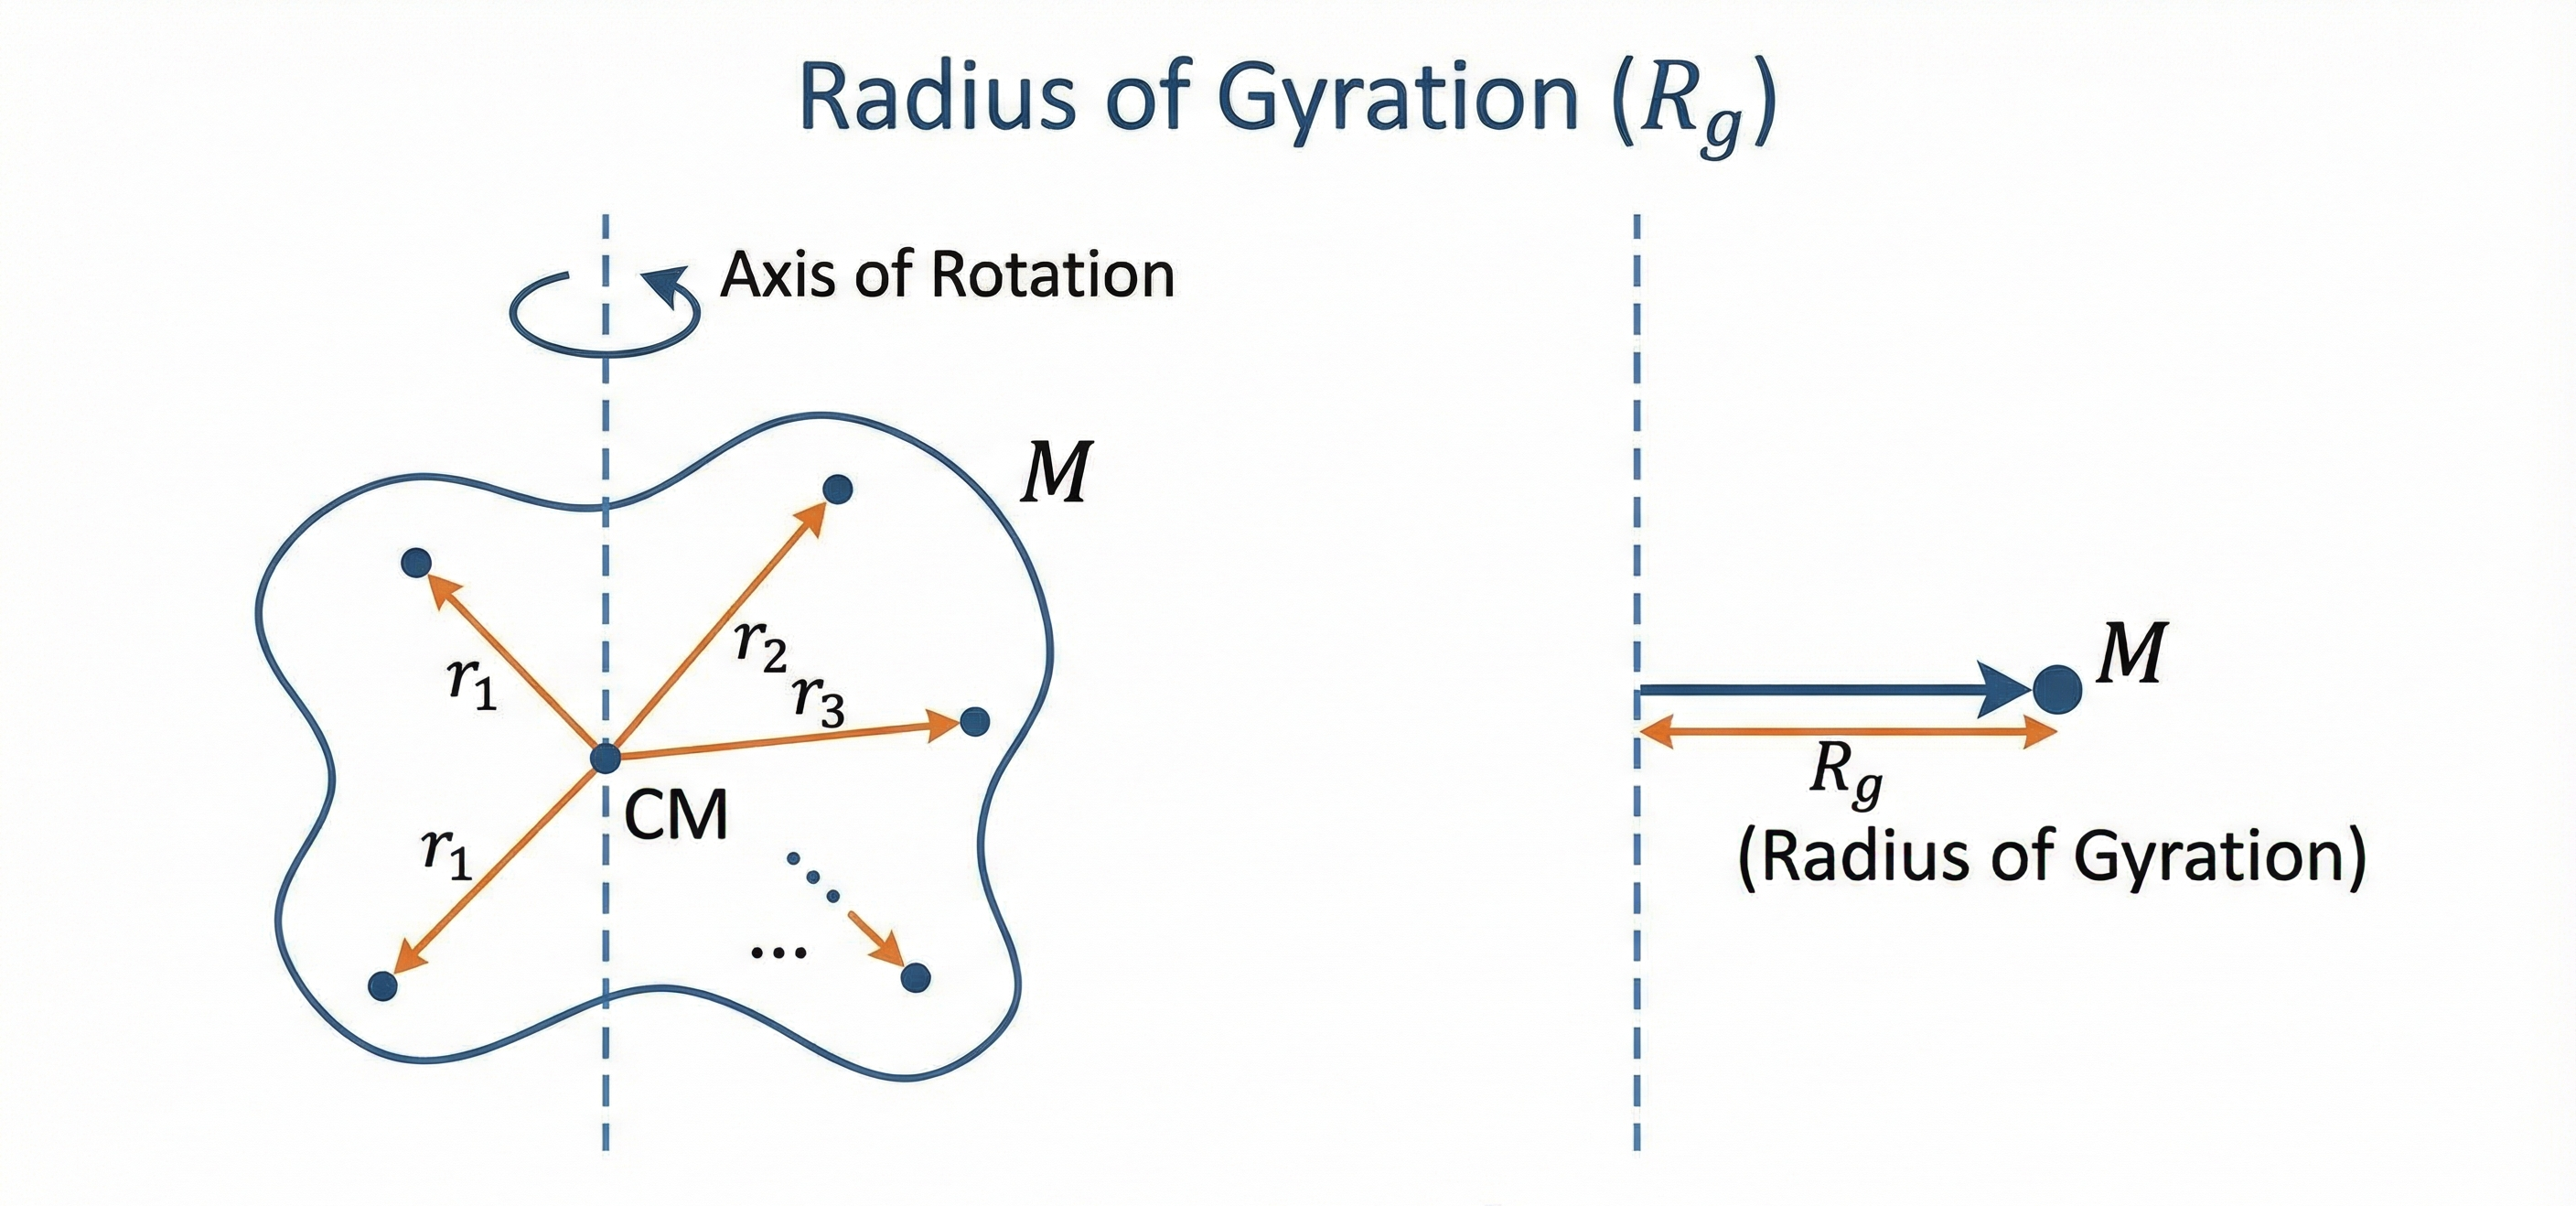
\includegraphics[width=0.6\textwidth]{img/radius_of_gyration.png}
    
    % Rövid cím (ábrajegyzékbe):
    \caption[A gyrációs sugár (Radius of Gyration) szemléltetése]{A gyrációs sugár ($r_g$) szemléltetése. \\ \footnotesize\textit{Forrás: AI generált kép}}
    
    % Hivatkozási címke:
    \label{fig:radius_gyration}
\end{figure}


A metrika eloszlása a populációban egy vágott hatványfüggvénnyel (truncated
power-law) közelíthető:
$P(r_{g}) \sim (r_{g}+r_{0})^{-\beta_r}\exp(-r_{g}/\kappa)$. González és munkatársai \cite{gonzalez2008understanding}
mérései alapján a jellemző paraméterek $r_{0} \approx 5{,}8$ km, $\beta_{r}\approx
1{,}65$ és a vágási érték $\kappa \approx 350$ km. A kutatások kimutatták, hogy az
$r_{g}$ időbeli növekedése csupán logaritmikus ütemű, ami arra utal, hogy az emberi
mozgás nem véletlenszerű diffúzió, hanem térben korlátozott és erősen visszatérő
jellegű \cite{gonzalez2008understanding}.






\subsection{Egyéb gyakori mobilitási metrikák}
\begin{itemize}
	\item \textbf{Látogatott egyedi helyek száma.} Egy adott időszakban
		meglátogatott különböző cellák számát $S$ jelöli. Nagy $S$ érték tág mozgási
		repertoárt jelez, míg kis $S$ koncentrált mozgást.

	\item \textbf{Napi/heti megtett távolság.} Az egymást követő cellák közötti
		távolságok összege. A metrika alulbecsülheti a tényleges útvonalat a pontos hely
		ismerete hiányában \cite{gonzalez2008understanding}.

	\item \textbf{Entrópia alapú mutatók.} A térbeli entrópia
		$H_{s} = -\sum_{j} p_{j} \log p_{j}$ a felhasználó cellalátogatási
		eloszlásából számítható, ahol $p_{j}$ a $j$-edik cella látogatási
		valószínűsége \cite{pinter2021evaluating}. A magas entrópia változatos térhasználatra,
		míg az alacsony érték kevés helyre koncentrálódó, kiszámítható mozgásra utal.
		\cite{pinter2022awakening}.

	\item \textbf{Home és work cella detektálása.} A leggyakoribb éjszakai hely az
		otthon, a Leggyakoribb nappali pedig a munkahely\cite{pinter2021evaluating, pinter2022awakening}

\end{itemize}

\subsection{Kiegészítő napi metrikák}
\label{subsec:extra_metrics}

A gyrációs sugár, az entrópia és a helydiverzitás mellett a CDR-szakirodalomban gyakran használt további napi metrikák, amelyeket a megvalósított rendszer (7.\ fejezet) szintén kiszámít:

\begin{itemize}
	\item \textbf{Aktivitáskoncentráció (AC).} A felhasználó napi pingjeinek hányadrésze esik a top~$k$ leglátogatottabb cellára:
		\[
		\mathrm{AC}_k = \frac{\sum_{j \in \mathrm{top}_k} n_j}{\sum_j n_j}, \qquad k = 3.
		\]
		Magas $\mathrm{AC}$ erősen koncentrált térhasználatot jelez. A korlátozó intézkedések (lockdown, vészhelyzet) tipikusan növelik az értékét \cite{pinter2022awakening}.

	\item \textbf{Visszatérési ráta (RR).} Az adott napon érintett cellák hányadrésze, amelyek az előző napon is érintettek voltak:
		\[
		\mathrm{RR}(d) = \frac{|C_d \cap C_{d-1}|}{|C_d|}, \qquad C_d = \{(x,y) \text{ cellák a } d \text{ napon}\}.
		\]
		Magas $\mathrm{RR}$ erős napi rutint, kiszámítható mozgást jelent. A González-féle visszatérő mozgásmodellel \cite{gonzalez2008understanding} áll rokonságban.

	\item \textbf{Csúcsidőrés (peak slot).} Az a 30~perces időrés ($t \in \{0,\dots,47\}$), amelyikben a felhasználó napi pingszáma maximális. A reggeli/esti ingázási csúcs \cite{pinter2022awakening} egyéni szintű proxyja.

	\item \textbf{Hétvége-jelző (weekend flag).} Bináris jelölő: $d \bmod 7 \in \{0, 6\}$ esetén hétvége. A hét napjainak sorrendjét empirikusan kell megállapítani, mert a YJMob100K nem hozza nyilvánosságra a kezdő dátumot (a levezetést a 9.\ fejezet validálja).
\end{itemize}

\clearpage
\section{OPEN-SOURCE CDR ADATHALOM BEMUTATÁSA}
% !TEX root = ../main.tex

A jelen fejezet a dolgozat empirikus részének alapját képező \textbf{YJMob100K} \cite{yabe2023metropolitan} adathalmazt mutatja be: az adatfelvétel körülményeit, a sémát, a két részadatkészlet közötti kapcsolatot, valamint a kísérő POI-fájlok szerepét. Az általános, kutatási célú CDR-adatkészletekre vonatkozó módszertani áttekintést a 3.7.\ szakasz tartalmazza.

\subsection{Az YJMob100K adatkészlet áttekintése}

Az YJMob100K adatkészletet Yabe és munkatársai \cite{yabe2023metropolitan} tették közzé 2023-ban a \emph{Scientific Data} folyóiratban, a HuMob Challenge mobilitás-előrejelzési verseny adatforrásaként. Az adatok a Yahoo Japan~Corporation egyik okostelefon-alkalmazásából (Yahoo Japan Application) származnak: anonimizált felhasználók eszközpozícióit rögzítik 30~perces időfelbontással, 75~napon át, egy 200$\times$200-as rácshálóra diszkretizálva. A megfigyelési terület közvetlenül nem nyilvános, ám térbeli sablonillesztéssel egyértelműen Nagoya nagyvárosi régiójához (Aichi prefektúra, Japán) köthető \cite{pinter2024revealing}.

Az adathalmaz Creative~Commons~BY 4.0 licenc alatt érhető el a Zenodo platformon\footnote{\url{https://zenodo.org/records/14219563}}. A dolgozat a \texttt{v3} adatverziót használja.

\begin{table}[H]
\centering
\caption{Az YJMob100K adatkészlet kulcsparaméterei.}
\label{tab:yjmob_summary}
\begin{tabular}{l l}
\hline
\textbf{Tulajdonság} & \textbf{Érték} \\
\hline
Forrás                  & Yahoo Japan Application, Yahoo Japan Corporation \\
Hivatkozás              & Yabe et al.\ \cite{yabe2023metropolitan} \\
Megfigyelési terület    & Nagoya, Aichi prefektúra, Japán \\
Időtartam               & 75~nap \\
Időfelbontás            & 30~perc (48~időrés/nap) \\
Térbeli felbontás       & 200$\times$200 cellás rács \\
Cellaméret (becsült)    & $\approx 455$~m (K--Ny) $\times \approx 556$~m (É--D) \\
Teljes kiterjedés       & $\approx 91$~km $\times \approx 111$~km \\
Felhasználók (dataset1) & 100~000 \\
Felhasználók (dataset2) & 25~000 (független kohorsz) \\
Rekordok (dataset1)     & 111\,535\,175 \\
Rekordok (dataset2)     &  29\,389\,749 \\
Összes rekord           & 140\,924\,924 \\
Licenc                  & CC~BY~4.0 \\
\hline
\end{tabular}
\end{table}

\subsection{Adatszerkezet}

Az alapadatfájlok (\path{yjmob100k-dataset1.csv}, \path{yjmob100k-dataset2.csv}) szerkezete azonos: minden sor egyetlen pingelési eseményt rögzít öt mezővel: \texttt{uid} (pszeudoanonim azonosító), \texttt{d} ($0\le d\le74$, megfigyelés napja), \texttt{t} ($0\le t\le47$, 30~perces időrés), \texttt{x}, \texttt{y} ($1\le x,y\le200$, rácskoordináták).

Fontos sajátosság, hogy az $x$ tengely a north--south (\textit{northing}) iránynak, az $y$ tengely az east--west (\textit{easting}) iránynak felel meg. Ez ellentétes a Descartes-koordináták szokásos $(x, y) = (\text{easting, northing})$ konvenciójával, és a feldolgozó kód minden ponton explicit módon kezeli (lásd 7.\ és 8.\ fejezet). Az adatfelvétel sem napszakot, sem dátumot nem rögzít közvetlenül; a hét napjainak ($d$~modulo~7) megfeleltetését empirikusan, az aktivitásmintázat heti periodicitásából vezettem le (lásd 9.7.\ szakasz).

\subsection{A két részadatkészlet közötti kapcsolat}
\label{subsec:two_datasets}

A Zenodo-adatközlés (v3) szerint a két fájl \emph{két diszjunkt felhasználói kohorszot} ír le ugyanazon a 75~napos időablakon és rácsterületen: a \texttt{dataset1} egy üzleti szokásrend szerinti („business-as-usual") populációt (100\,000~fő), a \texttt{dataset2} pedig egy ettől független, kisebb populációt (25\,000~fő) tartalmaz, amelynek utolsó 15~napját (\(d=60\ldots74\)) egy nem dokumentált kollektív viselkedési zavar (\enquote{vészhelyzet}) érinti.

Fontos figyelmeztetés: az \texttt{uid} mező mindkét fájlban 0-tól indul és \emph{kizárólag a saját fájljára érvényes} -- közös személyazonosítóként nem használható. A numerikus értékkészletek átfedése (\texttt{dataset2}: $0\ldots24\,999$ \(\subset\) \texttt{dataset1}: $0\ldots99\,999$) önmagában nem jelent személyazonosság-egyezést. Ezt empirikusan is ellenőriztem: a két fájl azonos \texttt{uid}-jeihez detektált otthoni cellák közül mindössze 2 esett egybe (a 23\,953 közös azonosítóból), az átlagos rácstávolságuk pedig $\approx 75$ cella ($\approx 38$~km), ami a véletlen-baseline ($\approx 104$ cella) közelében van. Ha a két fájl ugyanazokat a személyeket írná le, a home-cellák túlnyomó többségének egybe kéne esnie a tartózkodási hely napról-napra való stabilitása miatt.

Ennek két következménye van a módszertanra: (1) a vészhelyzet hatását \emph{populációszintű} (between-subject) összehasonlítással vizsgálom (\texttt{dataset1} baseline, \texttt{dataset2} kezelt; 7.4.\ és 9.5.\ szakasz); (2) az anomáliadetekciós modellt a \texttt{dataset1} normál mintáján tanítom és a \texttt{dataset2} vészhelyzeti időszakára alkalmazom, ahol a populációs heterogenitást kontrollálni kell (7.4.\ szakasz).

\subsection{Kísérő POI-fájlok}

Az adathalmaz két melléktáblát is tartalmaz: \texttt{cell\_POIcat.csv} (221\,000~sor; \texttt{(x, y, category, POI\_count)}) cellánkénti POI-kategória-eloszlással, és \texttt{POI\_datacategories.csv} (85~sor) a kategórianevek feloldásával (pl.\ \emph{Bakery}, \emph{Hospital}, \emph{Transit Station}).

A 85 finomszemcsés POI-kategóriát a \texttt{schema.py} 9 magasabb szintű \textbf{zónába} (\textit{food, shopping, leisure, transit, parking, healthcare, education, services, industry}) sorolja össze, amely táblát a \texttt{dim\_cell} dimenzió-tábla \texttt{poi\_zone} oszlopa tartalmazza. A teljes leképezés a \emph{Függelék}~A.1.\ alatt található.

\subsection{Adatminőségi és értelmezési megfontolások}

Az YJMob100K, mint minden anonimizált CDR-jellegű adathalmaz, a 3.7.\ szakaszban felsorolt általános korlátokon túl néhány specifikus megfontolást igényel: \textbf{reprezentativitás} (kizárólag a Yahoo Japan Application felhasználói, fiatalabb többséggel); \textbf{térbeli felbontás} (a névleges 500~m megtévesztő, valódi cellaméretek $\approx 454{,}5 \times 555{,}6$~m); \textbf{időbeli horgonyzás hiánya} (csak relatív heti/napi mintázatok); \textbf{esemény-jellegű hiányosság} (a vészhelyzet típusa rejtett, az anomália csak strukturálisan értelmezhető).

A korlátok ellenére az YJMob100K az egyik legnagyobb, nyíltan elérhető nagyvárosi mobilitási adatkészlet, amelynek mérete (141~M rekord) és időbeli mélysége (75~nap) a CDR-szakirodalomban szokásosnál is részletesebb elemzéseket tesz lehetővé.


\clearpage
\section{RENDSZERTERV A CDR ADATOK FELDOLGOZÁSÁRA ÉS TÁROLÁSÁRA}
% !TEX root = ../main.tex

A jelen fejezetben bemutatom a CDR adatfeldolgozó rendszer tervezési döntéseit: milyen technológiai alternatívákat mérlegeltem, és az adott korlátok mellett miért az alábbi eszközöket választottam. A rendszer célja a YJMob100K adathalom (5.\ fejezet) feldolgozása, a 4.\ fejezetben ismertetett mobilitási metrikák kiszámítása, valamint a származtatott mutatók GIS alapú megjelenítése.

\subsection{Tervezési szempontok és korlátok}

A rendszerterv kialakítását három fő szempont határozta meg:
\begin{enumerate}
    \item \textbf{Adatméret:} A YJMob100K adathalom két fő CSV fájlja összesen mintegy 141~millió sort tartalmaz. Az adatbázis-motornak képesnek kell lennie ennyi rekord hatékony kezelésére anélkül, hogy a teljes adatot a memóriába kellene tölteni.
    \item \textbf{Hardverkorlátok:} A fejlesztő gép 16~GB RAM-mal és 6 magos Intel i5-8400 processzorral rendelkezik. Elosztott cluster nem áll rendelkezésre, így a választott eszközöknek egyetlen gépen is hatékonynak kell lenniük.
    \item \textbf{Reprodukálhatóság:} A teljes pipeline-nak szkriptelhetőnek, verziókezelhetőnek és parancssori futtatással újrafuttathatónak kell lennie, külső szerver vagy GUI nélkül.
\end{enumerate}

\subsection{Technológiai alternatívák értékelése}

Az alábbiakban áttekintem az egyes funkcióterületek mérlegelt alternatíváit, és megindokolom a végső választást.

\subsubsection{Adatbázis-motor}

A CDR feldolgozás irodalmában a relációs adatbázisok (PostgreSQL, Microsoft SQL Server), az elosztott big-data rendszerek (Apache Spark + Hadoop HDFS), valamint az újabb beágyazott OLAP megoldások (DuckDB, SQLite) fordulnak elő \cite{zhang2019connected, pinter2020artificial}.

\begin{itemize}
    \item \textbf{PostgreSQL / PostGIS} -- széles körben használt nyílt forráskódú relációs adatbázis, amely a PostGIS kiterjesztéssel natív térbeli indexelést és GIS-funkciókat nyújt. Hátránya, hogy külön szerverfolyamatot igényel, és a 141 millió soros OLAP jellegű aggregációknál (teljes tábla átlagolása, GROUP BY a teljes adaton) sor-orientált tárolása miatt lassabb, mint egy oszlopos motor.
    \item \textbf{Apache Spark} -- elosztott számítási keretrendszer, amely a szakirodalomban gyakori választás CDR feldolgozásra \cite{zhang2019connected}. Legnagyobb előnye a horizontális skálázhatóság, azonban egyetlen gépen a JVM-alapú futtatókörnyezet magas memóriaigénye és a konfigurációs komplexitás nem indokolt.
    \item \textbf{DuckDB} -- beágyazott (in-process), oszlopos OLAP adatbázis-motor, amely közvetlenül a Python folyamatba integrálódik. Nem igényel szervertelepítést, a CSV fájlokat streaming módban olvassa (nem kell a teljes adat a memóriában), és a vektorizált végrehajtó motorja révén a százmilliós aggregációk is másodpercek alatt futnak 16~GB RAM mellett.
\end{itemize}

A \textbf{DuckDB} mellett döntöttem, mivel az adathalom ugyan nagy, de egyetlen gépre fér; az oszlopos tárolás és a vektorizált végrehajtás ideális a mobilitási metrikák GROUP BY-intenzív SQL lekérdezéseihez; és a Python API-n keresztül közvetlenül pandas DataFrame-ekké alakíthatók az eredmények. Az SQL nyelv használata azt is biztosítja, hogy a lekérdezések a jövőben más motoron (pl.\ PostgreSQL) is futtathatók maradjanak.

\subsubsection{Programozási nyelv és ETL megközelítés}

A feldolgozó pipeline nyelveként \textbf{Python} volt a természetes választás, mivel az adatelemzési ökoszisztéma (pandas, scikit-learn, matplotlib) egységes keretet biztosít az ETL, a gépi tanulás és a vizualizáció számára. Alternatívaként felmerülő R-nyelv GIS-támogatása kevésbé kiforrott, az SSIS (SQL Server Integration Services) pedig zárt forráskódú és platformfüggő.

Az ETL logikát közvetlenül Python szkriptekbe szerveztem, modul-szintű felelősségmegosztással. Egy-egy szkript egy-egy pipeline-fázist valósít meg, és a parancssorból futtatható. A köztes eredményeket Parquet formátumban is exportálom, ami hatékony oszlopos tárolást biztosít és biztonsági mentésként is szolgál.

\subsubsection{Térbeli feldolgozás (GIS)}

A GIS komponens feladata a YJMob100K rácskoordinátáinak georeferálása és térképes megjelenítése. A mérlegelt alternatívák:
\begin{itemize}
    \item \textbf{QGIS} -- asztali GIS alkalmazás, amely manuális rétegkezelést és interaktív térképszerkesztést kínál. Hátránya, hogy a munkafolyamat nehezen szkriptelhető és nem reprodukálható automatikusan.
    \item \textbf{PostGIS} -- a PostgreSQL térbeli kiterjesztése; erős a térbeli lekérdezésekben, de külön adatbázis-szervert igényel, és a vizualizációhoz további eszköz (pl.\ QGIS) szükséges.
    \item \textbf{GeoPandas + pyproj + contextily} -- Python könyvtárcsalád, amely programozottan végzi a koordináta-transzformációkat, GeoDataFrame-eket kezel, és OpenStreetMap alaptérképekre rajzol. Teljes mértékben szkriptelhető és a Jupyter Notebook-okba integrálható.
\end{itemize}

A \textbf{GeoPandas + pyproj} kombinációt választottam: a pyproj a koordináta-transzformációt végzi (EPSG:2449 $\rightarrow$ WGS84), a GeoPandas a térbeli adatszerkezeteket kezeli, a contextily pedig az OpenStreetMap csemperéteget biztosítja alaptérképként. Ez a megoldás lehetővé teszi, hogy a teljes GIS munkafolyamat Python kódból futtatható és reprodukálható legyen.

\subsubsection{Anomáliadetekció}

A rendszerterv része a viselkedési anomáliák felismerése is, amelyet az adatkészlet második részének vészhelyzeti időszaka (60--74.\ nap) tesz lehetővé. A scikit-learn könyvtár Isolation Forest algoritmusát választottam, mivel felügyelet nélküli módszer (nem igényel címkézett adatot), jól skálázódik a többszázezres mintaméretre, és a Python ökoszisztéma részét képezi.

\subsubsection{Vizualizáció}

A vizualizációhoz a \textbf{matplotlib + seaborn} párost választottam a statikus, tudományos minőségű ábrák elkészítéséhez. Az interaktív megoldásokat (Plotly, Folium, kepler.gl) mérlegeltem, de a dolgozat célja nyomtatott minőségű ábrák előállítása, amelyhez a matplotlib jobban illeszkedik. A kontextushoz az OpenStreetMap alaptérképeket a contextily könyvtár biztosítja.

\subsection{A választott technológiai stack összefoglalása}

Az alábbi táblázat foglalja össze az egyes rétegek kiválasztott eszközeit:

\begin{table}[H]
\centering
\caption{A megvalósított rendszer technológiai stack-je.}
\label{tab:tech_stack}
\begin{tabular}{l l l}
\hline
\textbf{Réteg} & \textbf{Eszköz} & \textbf{Szerep} \\
\hline
Adatbázis       & DuckDB            & Oszlopos OLAP, in-process \\
ETL nyelv       & Python            & Pipeline szkriptek \\
Adathíd         & pandas            & Python $\leftrightarrow$ DuckDB \\
Georeferálás    & pyproj            & EPSG:2449 $\rightarrow$ WGS84 \\
Térbeli adat    & GeoPandas         & GeoDataFrame kezelés \\
Alaptérkép      & contextily        & OpenStreetMap csempék \\
Anomáliadetekció & scikit-learn     & Isolation Forest \\
Ábrák           & matplotlib, seaborn & Statikus vizualizáció \\
Köztes formátum & Parquet           & Oszlopos export/mentés \\
\hline
\end{tabular}
\end{table}


\subsection{Magasszintű architektúra}

A rendszer négy fő rétegből áll (\autoref{fig:arch}):

\begin{enumerate}
    \item \textbf{Adatforrás réteg.} A nyers CSV fájlok (YJMob100K dataset1, dataset2) és a kiegészítő adatok (POI kategóriák). Ezeket a DuckDB \texttt{read\_csv} streaming olvasója dolgozza fel, tehát a teljes CSV soha nem kerül egyben a memóriába.

    \item \textbf{Perzisztens tároló (DuckDB).} A betöltött adatok DuckDB táblákba kerülnek, amelyek oszlopos formátumban, tömörítve tárolódnak egyetlen fájlban (\texttt{mobility.duckdb}). Ez egyben a Data Warehouse szerepet is betölti, mivel a dimenziós táblákat is itt hozom létre.

    \item \textbf{Analitikai réteg.} A mobilitási metrikákat SQL CTE-láncokon (Common Table Expression) keresztül számítom ki a DuckDB-ben, majd az eredményeket Parquet fájlokba is exportálom. Az anomáliadetekciót a scikit-learn végzi Python-ban, a DuckDB-ből kiolvasott feature mátrixon.

    \item \textbf{Megjelenítési réteg.} A származtatott mutatókat a GeoPandas georeferálja, a matplotlib + contextily pedig térképes és statisztikai ábrákon jeleníti meg.
\end{enumerate}

\begin{figure}[H]
\centering
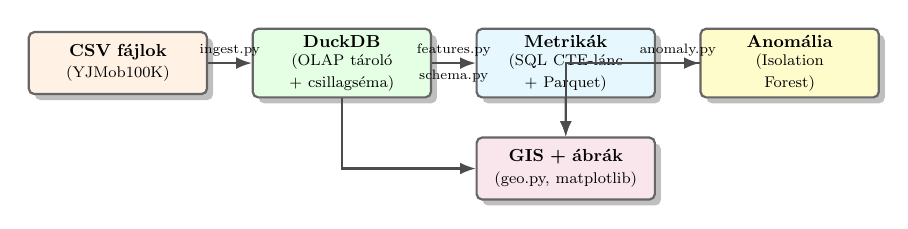
\begin{tikzpicture}[
    scale=0.70,
    transform shape,
    node distance=0.8cm,
    auto,
    block/.style={
        rectangle,
        draw=black!60,
        fill=blue!5,
        thick,
        text width=3.0cm,
        align=center,
        font=\small,
        rounded corners=2pt,
        minimum height=3.2em,
        drop shadow
    },
    arrow/.style={
        -{Latex[length=2mm]},
        thick,
        draw=black!70
    }
]
    \node [block, fill=orange!10] (step1) {\textbf{CSV fájlok}\\ \footnotesize(YJMob100K)};
    \node [block, right=of step1, fill=green!10] (step2) {\textbf{DuckDB}\\ \footnotesize(OLAP tároló \\ + csillagséma)};
    \node [block, right=of step2, fill=cyan!10] (step3) {\textbf{Metrikák}\\ \footnotesize(SQL CTE-lánc \\ + Parquet)};
    \node [block, right=of step3, fill=yellow!20] (step4) {\textbf{Anomália}\\ \footnotesize(Isolation \\ Forest)};
    \node [block, below=0.7cm of step3, fill=purple!10] (step5) {\textbf{GIS + ábrák}\\ \footnotesize(geo.py, matplotlib)};

    \draw [arrow] (step1) -- node[above, font=\scriptsize]{ingest.py} (step2);
    \draw [arrow] (step2) -- node[above, font=\scriptsize]{features.py} node[below, font=\scriptsize]{schema.py} (step3);
    \draw [arrow] (step3) -- node[above, font=\scriptsize]{anomaly.py} (step4);
    \draw [arrow] (step2) |- (step5);
    \draw [arrow] (step3) -- (step5);
    \draw [arrow] (step4) -| (step5);
\end{tikzpicture}
\caption{A megvalósított CDR feldolgozó rendszer magas szintű architektúrája. A négy ETL-fázis (ingest $\to$ features/schema $\to$ anomaly) a DuckDB tárolón keresztül kommunikál; a megjelenítési réteg (\texttt{geo.py} + matplotlib) közvetlenül olvassa a DuckDB-t és a Parquet outputokat.}
\label{fig:arch}
\end{figure}

\subsection{Adatbázis-terv: csillagséma}

Az adatbázis logikai modellje csillagsémára épül, amelyet a 3.\ fejezetben bemutatott általános CDR adatmodellből vezettem le, a YJMob100K sajátosságaihoz igazítva.

A \textbf{ténytáblák} a nyers mobilitási rekordokat tartalmazzák:
\begin{itemize}
    \item \textbf{mobility1} -- a normál időszak 111{,}5~millió rekordja (100~000 felhasználó, 75 nap).
    \item \textbf{mobility2} -- a vészhelyzeti időszak 29{,}4~millió rekordja (25\,000 felhasználó, 75 nap, ebből az utolsó 15 nap rendkívüli). A két adatkészlet független kohorsz, így a teljes felhasználószám $100\,000 + 25\,000 = 125\,000$ (a részleteket lásd az 5.3.\ szakaszban).
\end{itemize}

\noindent Minden rekord öt mezőből áll: \texttt{uid} (előfizető), \texttt{d} (nap), \texttt{t} (30~perces időrés), \texttt{x} és \texttt{y} (rácskoordináták).

A \textbf{dimenzió táblák}:
\begin{itemize}
    \item \textbf{dim\_time} -- az időrések metaadatai: a \texttt{(d, t)} párból számított óra, napszak (éjszaka/reggel/délután/este), hét napja, hétköznap/hétvége jelző, valamint a vészhelyzeti időszak jelölése (d $\geq$ 60). Összesen 3\,600 sor ($75 \times 48$).
    \item \textbf{dim\_cell} -- a rácscellákon számított térbeli attribútumok: domináns POI kategória, zónatípus (élelmiszer, bevásárlás, közlekedés stb.), összesített POI szám. Csak azok a cellák szerepelnek, amelyekben tényleges aktivitás volt (20\,146 sor a 40\,000-ből).
    \item \textbf{dim\_user} -- felhasználói összefoglaló: az adatkészlet azonosítója, becsült otthon- és munkahely-cella, otthon--munkahely távolság. Természetes kulcs: \((\texttt{uid}, \texttt{dataset})\) kompozit kulcs, mivel a két adatkészlet független kohorsz (lásd 5.3.\ szakasz). 121\,607 sor (a 125\,000 felhasználóból ennyihez sikerült stabil otthoncellát hozzárendelni). A felhasználói archetípus-klaszterezés (lásd 9.6.\ szakasz) eredménye nem a dimenzió-táblában, hanem külön \texttt{output/user\_archetypes.csv} fájlban tárolódik, hogy az analitikai modellfuttatások függetlenek maradjanak az adatraktártól.
\end{itemize}

\noindent A származtatott mobilitási metrikákat két aggregált tábla tárolja (\texttt{user\_daily\_features1} és \texttt{user\_daily\_features2}), amelyeket a 4.\ fejezetben bemutatott képletek alapján SQL-ben számítok ki. Ezek felhasználónként és naponként tartalmazzák a gyrációs sugarat, a Shannon-entrópiát, a lokációs diverzitást, a becsült otthon- és munkahely-cellát, valamint az otthon--munkahely távolságot méterben.

\subsection{Feldolgozási folyamat (pipeline)}

A feldolgozást négy, parancssorból egymás után futtatható Python modulra bontom; a köztes adatáramlást a központi \texttt{mobility.duckdb} fájl és Parquet exportok biztosítják. Az egyes fázisok bemenete--kimenete a \autoref{tab:pipeline_phases} táblázatban szerepel; a tényleges implementáció részleteit (kódminták, futási idők) a 7.\ fejezet tárgyalja.

\begin{table}[H]
\centering
\caption{A pipeline négy fázisa, modulok és inputok/outputok.}
\label{tab:pipeline_phases}
\begin{tabular}{l l p{4.5cm} p{4.5cm}}
\hline
\textbf{\#} & \textbf{Modul} & \textbf{Bemenet} & \textbf{Kimenet} \\
\hline
1 & \texttt{ingest.py}   & 4 db CSV (YJMob100K) & 4 DuckDB tábla (\texttt{mobility1/2}, \texttt{cell\_poi\_cat}, \texttt{poi\_categories}) \\
2 & \texttt{features.py} & \texttt{mobility1/2} & \texttt{user\_daily\_features1/2} (DuckDB + Parquet) \\
3 & \texttt{schema.py}   & ténytáblák, POI-tábla & \texttt{dim\_time}, \texttt{dim\_cell}, \texttt{dim\_user} \\
4 & \texttt{anomaly.py}  & \texttt{user\_daily\_features1/2} & \texttt{anomaly\_scores*.parquet} \\
\hline
\end{tabular}
\end{table}

\subsection{Georeferálási megoldás}

Az YJMob100K 200$\times$200-as rácsa önmagában nem hordoz földrajzi információt. A rácsot az EPSG:2449 (Japan Plane Rectangular CS~VII) vetületi koordináta-rendszerbe helyeztem el a \texttt{reverse-engineering-YJMob100K-grid} projekt \cite{pinter2024revealing} eredményei alapján; a vetületi koordináták WGS84-re való átváltását a pyproj \texttt{Transformer} osztálya végzi a \texttt{geo.py} modulban. A rácsparaméterek (origó, anizotrop cellaméretek, tengelykonvenció) és a tényleges implementáció részleteit a 8.\ fejezet tárgyalja.

\subsection{Kockázatok és korlátok}

A rendszerterv megvalósítása során a következő korlátokkal számoltam:
\begin{itemize}
    \item \textbf{Térbeli pontosság:} A rács cellamérete (${\sim}455 \times 556$~m) durvábbá teszi a pozíciómeghatározást, mint egy valódi bázisállomás-hálózat városi részén. A metrikák így a rácsszintű felbontásra vonatkoznak \cite{gonzalez2008understanding}.
    \item \textbf{Georeferálás bizonytalansága:} A rácsparamétereket inverz mérnöki módszerrel határoztam meg; az origó pontos helye néhány száz méteres bizonytalansággal terhelt.
    \item \textbf{Anomáliadetekció validálása:} Felügyelet nélküli módszert alkalmazok (Isolation Forest), amelynek kiértékelése címkézett ground truth adat hiányában korlátozott. Az eredményeket a vészhelyzeti időszak ismert kontextusa alapján értékelem.
\end{itemize}


\clearpage
\section{IMPLEMENTÁCIÓ}
% !TEX root = ../main.tex

A jelen fejezetben a 6.\ fejezetben megtervezett rendszer tényleges megvalósítását mutatjuk be. A pipeline négy egymásra épülő Python szkriptből áll; mindegyik egy jól körülhatárolt fázist valósít meg, és a projekt gyökérkönyvtárából futtatható.

\subsection{Az adatbetöltési fázis}

Az \texttt{ingest.py} felelős a nyers CSV fájlok DuckDB adatbázisba töltéséért. Az adatbázis-kapcsolat létrehozásakor az elérhető processzormagokhoz (6~mag) és a rendelkezésre álló memóriához (10~GB-os limitet állítunk be) igazítjuk a DuckDB szálkezelését:

\begin{lstlisting}[language=Python, caption={DuckDB kapcsolat konfigurálása.}, label={lst:connect}, basicstyle=\small\ttfamily, breaklines=true, frame=single]
con = duckdb.connect(str(DB_PATH))
con.execute("SET threads TO 6")
con.execute("SET memory_limit = '10GB'")
\end{lstlisting}

A CSV fájlok betöltése a DuckDB beépített \texttt{read\_csv} függvényével történik, streaming módban: a teljes fájl soha nem kerül egyszerre a memóriába. Az oszlopok explicit típusmegjelölést kapnak (pl.\ \texttt{UINTEGER}, \texttt{UTINYINT}, \texttt{USMALLINT}), ezzel minimalizálva a memóriahasználatot az automatikus típusbecsléshez képest:

\begin{lstlisting}[language=SQL, caption={A \texttt{mobility1} tábla létrehozása streaming CSV-olvasással.}, label={lst:mobility_load}, basicstyle=\small\ttfamily, breaklines=true, frame=single]
CREATE TABLE mobility1 AS
SELECT * FROM read_csv(
    'yjmob100k-dataset1.csv',
    columns = {
        'uid': 'UINTEGER',  'd': 'UTINYINT',
        't':   'UTINYINT',  'x': 'USMALLINT',
        'y':   'USMALLINT'
    },
    header = true
)
\end{lstlisting}

A betöltés végén sorszám-validáció ellenőrzi, hogy az elvárt sorok mind bekerültek. Az alábbi táblázat foglalja össze a betöltött táblákat (\autoref{tab:loaded_tables}):

\begin{table}[H]
\centering
\caption{A DuckDB adatbázisba betöltött táblák és sorszámaik.}
\label{tab:loaded_tables}
\begin{tabular}{l r l}
\hline
\textbf{Tábla} & \textbf{Sorok száma} & \textbf{Tartalom} \\
\hline
\texttt{mobility1}       & 111~535~175 & Normál időszak (100~000 felhasználó, 75~nap) \\
\texttt{mobility2}       &  29~389~749 & Vészhelyzeti időszak (25~000 felhasználó, 75~nap) \\
\texttt{cell\_poi\_cat}  &    221~000  & POI-kategória rácscelláként \\
\texttt{poi\_categories} &         85 & POI-kategória megnevezések \\
\hline
\textbf{Összesen}        & 140~924~924 & \\
\hline
\end{tabular}
\end{table}

\subsection{Mobilitási metrikák számítása}

A \texttt{features.py} CTE-láncolatot (\textit{Common Table Expression}) alkalmaz: minden egyes metrika egy-egy SQL CTE-ben kerül kiszámításra, és a záró \texttt{SELECT} összekapcsolja azokat. Ez az architektúra áttekinthetővé teszi a lekérdezést, és a DuckDB optimalizálója a több logikai lépést egyetlen vektorizált végrehajtási tervvé fordítja le.

A CTE-lánc hat egységből áll:

\begin{enumerate}
\item \textbf{base}: felhasználónként és naponként kiszámítja az összes ping számát (\texttt{total\_pings}) és a napi centroid koordinátáit ($c_x$, $c_y$).
\item \textbf{diversity}: az egyedi cellakoordináta-párok száma (\texttt{location\_diversity}). Az egyediséget az $x \cdot 201 + y$ hash-kulccsal azonosítjuk, amely egyértelműen megkülönbözteti a 200×200-as rács összes celláját.
\item \textbf{entropy}: a Shannon-entrópia kiszámítása $-\sum p_i \log_2 p_i$ képlettel, ahol $p_i$ az $i$-edik cella látogatási valószínűsége.
\item \textbf{rog}: a gyrációs sugár kiszámítása anizotrop cellaméretekkel (easting: $\approx 454{,}5$~m, northing: $\approx 555{,}6$~m). A két iránybeli eltérő cellaméret figyelembevétele nélkül a sugár torzított lenne:

\begin{lstlisting}[language=SQL, caption={A gyrációs sugár SQL-implementációja anizotrop cellaméretekkel.}, label={lst:rog}, basicstyle=\small\ttfamily, breaklines=true, frame=single]
SQRT(AVG(
    POWER((m.x::DOUBLE - b.cx) * 555.556, 2) +
    POWER((m.y::DOUBLE - b.cy) * 454.545, 2)
)) AS radius_of_gyration
\end{lstlisting}

\item \textbf{home}: az éjszakai időrések ($t = 0\ldots11$, azaz 00:00--05:59) leggyakoribb celláját tekintjük otthonnak; az \texttt{ROW\_NUMBER()} ablakfüggvény biztosítja, hogy minden (uid, d) párhoz pontosan egy érték kerüljön ki.
\item \textbf{work}: a 08:00--14:00 közötti munkaidős időrések ($t = 16\ldots28$) domináns cellája; a home--work távolságot euklideszi képlettel számítjuk a vetületi méterértékekből.
\end{enumerate}

A számítás eredménye 7{,}1~millió sor (dataset1) és 1{,}8~millió sor (dataset2), amelyeket a rendszer DuckDB táblában és Parquet fájlban is tárol.

\subsection{A csillagséma kialakítása}

A \texttt{schema.py} három dimenzió-táblát hoz létre az adatbázisban.

\textbf{dim\_time} (3~600~sor): a 75~nap × 48~időrés minden kombinációjához tartalmaz metaadatot: az óra számát, a napszakot (\textit{night / morning / afternoon / evening}), a hét napját (\texttt{dow}), az \texttt{is\_weekday} logikai jelzőt, valamint a \texttt{period\_label} oszlopot, amely megkülönbözteti az alap- (\textit{baseline}) és a vészhelyzeti (\textit{emergency}) időszakot. A hét napjának megállapításakor a $d = 0$ értéket vasárnaphoz rendeltük, amit az aktivitásmintázat heti periodicitása alapján vezettünk le.

\textbf{dim\_cell} (20~146~sor): az aktív rácscellákat (legalább egy ping-gel rendelkezőket) tartalmazza a domináns POI-kategóriával és egy összevont zónabesorolással. A 85 POI-kategóriát szabályalapú leképezéssel rendeljük 9 zónához: élelmezés, kereskedelem, szabadidő, közlekedés, parkolás, egészségügy, oktatás, szolgáltatás és ipar. A zónatérkép célja az elemzések értelmezhetőségének javítása.

\textbf{dim\_user} (121\,607~sor): minden \texttt{(uid, dataset)} kombinációhoz tartalmaz egy sort a detektált otthon- és munkahely-cellával, valamint az otthon--munkahely távolsággal. A két adatkészlet független felhasználói kohörsz (lásd 5.3.\ szakasz), így az \texttt{uid} önmagában nem természetes kulcs --- a táblát \((\texttt{uid}, \texttt{dataset})\) kompozit kulcs azonosítja. A 125\,000 felhasználóból (dataset1: 100\,000; dataset2: 25\,000) 121\,607-hez sikerült otthoncellát hozzárendelni; a fennmaradó $\approx 3\,400$ felhasználó nem rendelkezik elegendő éjszakai ($t = 0\ldots11$) ping-aktivitással a stabil otthon-detekcióhoz.

\subsection{Anomáliadetekció}

Az \texttt{anomaly.py} Isolation Forest algoritmust \cite{liu2008isolation} alkalmaz a viselkedési rendellenességek azonosítására. A tanítás a dataset1 összes rekordjára (normál viselkedés) történik, a pontszámozás pedig a dataset2 vészhelyzeti időszakán ($d \geq 60$) fut.

A feature-mátrix öt jellemzőből áll: \texttt{total\_pings}, \texttt{location\_diversity}, \texttt{shannon\_entropy}, \texttt{radius\_of\_gyration} és \texttt{home\_work\_dist\_m}. A StandardScaler normalizálja az értékeket a tanítás előtt, mivel a jellemzők különböző skálákon mozognak (pl.\ ping-szám vs.\ méter).

Az Isolation Forest paraméterei: 200 döntési fa (\texttt{n\_estimators = 200}), konzervatív szennyezettség (\texttt{contamination = 0.05}) és rögzített véletlenszám-mag (\texttt{random\_state = 42}) a reprodukálhatóság érdekében. A modell kimenete az \texttt{anomaly\_scores.parquet} fájlba kerül, amely minden (uid, d) párhoz tartalmazza az anomáliapontszámot és az \texttt{is\_anomaly} logikai jelzőt.

\subsection{Tesztelés, validáció és teljesítménymérés}
\label{subsec:validation}

A megvalósított pipeline működését két szinten ellenőriztük: (i) sor- és sémaintegritási vizsgálatokkal a betöltés és a csillagséma építése során, valamint (ii) reprezentatív lekérdezések futási idejének mérésével. A felhasználói kohorszok diszjunkt jellegének kvantitatív igazolása (23\,953 közös \texttt{uid}-ből 2 egyező otthoncella) a \autoref{subsec:two_datasets}.\ szakaszban szerepel, ide nem ismételjük meg.

\subsubsection{Sor- és sémavalidáció}

Az \texttt{ingest.py} a betöltés után minden táblára ellenőrzi a sorszámot a CSV-ből előre meghatározott értékkel összevetve (\autoref{tab:loaded_tables}). A \texttt{schema.py} a dimenziók építése után hasonlóan ellenőrzi: a \texttt{dim\_time} pontosan $75 \times 48 = 3\,600$ sort, a \texttt{dim\_cell} kizárólag aktív (POI-bejegyzéssel rendelkező) cellákat, a \texttt{dim\_user} pedig (\texttt{uid, dataset}) szerint egyedi kombinációkat tartalmaz.

\subsubsection{Lekérdezési teljesítmény}

Reprezentatív lekérdezések futási idejét az \autoref{tab:perf} foglalja össze (DuckDB v1.4, 6~mag, 10~GB memórialimit, 3~000~MB-os adatbázisfájl). A 111~M soros \texttt{mobility1} \texttt{GROUP BY (uid, d)} aggregációja $\approx 3{,}7$ másodperc alatt végez --- ez igazolja a 6.\ fejezetben leírt választást: oszlopos tárolás és vektorizált végrehajtás mellett a 141~M soros adathalom egyetlen 16~GB-os gépen, interaktív időablakban feldolgozható.

\begin{table}[H]
\centering
\caption{Reprezentatív DuckDB-lekérdezések futtatási ideje (saját mérés).}
\label{tab:perf}
\begin{tabular}{l r r}
\hline
\textbf{Lekérdezés} & \textbf{Eredmény-sorok} & \textbf{Idő (s)} \\
\hline
\texttt{COUNT(*)} \texttt{mobility1} (111~M sor)            &           1 & 0{,}01 \\
\texttt{COUNT(*)} \texttt{mobility2} (29~M sor)             &           1 & $<\!0{,}01$ \\
\texttt{GROUP BY uid} aggregáció \texttt{mobility1}-en      &     100\,000 & 0{,}69 \\
\texttt{GROUP BY (uid,d)} aggregáció \texttt{mobility1}-en  &  7\,147\,619 & 3{,}69 \\
\texttt{JOIN dim\_cell} \texttt{(x,y)} szerint, POI-zonánként &           9 & 1{,}07 \\
\texttt{user\_daily\_features1} olvasás + \texttt{AVG}      &           1 & 0{,}01 \\
\hline
\end{tabular}
\end{table}

\subsubsection{Anomáliadetekció stabilitása}

A rögzített \texttt{random\_state = 42} determinisztikus reprodukálhatóságot biztosít: az \texttt{anomaly.py} ismételt futtatásai bitre azonos \texttt{anomaly\_scores.parquet} fájlt állítanak elő. Címkézett ground-truth hiányában a modell kvalitatív validációját az anomálisnak minősített felhasználók szignifikánsan magasabb mobilitási mutatói adják (gyrációs sugár 4{,}52$\times$, otthon--munkahely távolság 10{,}98$\times$, lásd \autoref{tab:anomaly_comparison}).


\clearpage
\section{GIS-ALAPÚ TÉRBELI MEGJELENÍTÉS}
% !TEX root = ../main.tex

A jelen fejezet az YJMob100K adathalmaz rácskoordinátáinak georeferálását és térképes megjelenítését mutatja be. A vizualizáció OpenStreetMap alaptérképre vetítve, pyproj-alapú koordináta-transzformációval készült.

\subsection{Georeferálási módszertan}

Az YJMob100K adathalmaz nem hozza nyilvánosságra a mérési helyszínt; az adatrekordok koordinátái 1--200 közötti rácsindexek, nem geodéziai koordináták. A rács valós térbeli elhelyezkedéséhez a \textit{reverse-engineering-YJMob100K-grid} projekt \cite{pinter2024revealing} eredményeit alkalmaztam, amely sablonillesztéssel azonosította a megfigyelési területet Nagoya városával (Aichi prefektúra, Japán).

A meghatározott koordináta-rendszer az EPSG:2449 (Japan Plane Rectangular CS~VII), amelynek origója 36°~északi szélesség és 137°~35'~keleti hosszúság. Az adatkészletben az $x$ tengelyindex az észak--déli (\textit{northing}), az $y$ index a kelet--nyugati (\textit{easting}) irányba növekszik (lásd 5.~fejezet).

Ellentétben a névleges 500~m-es rácsmérethivatkozással, a cellák nem négyzetesek: az easting irányú méret $5000 / 11 \approx 454{,}5$~m, a northing irányú méret $5000 / 9 \approx 555{,}6$~m. Az 5.\ fejezetben jelzett aszimmetria elkerülésére a \texttt{features.py} mindkét értéket explicit módon alkalmazza (ld.\ 7.\ fejezet).

A rács sarokpontja (az $(1, 1)$ cella bal alsó sarka) EPSG:2449-ben: easting $= {-60\,682}$~m, northing $= {-166\,667}$~m. Az ebből levezetett teljes kiterjedés: $\approx 91$~km (kelet--nyugat) × $\approx 111$~km (észak--dél).

\subsection{Megvalósítás}

A georeferálást a \texttt{geo.py} modul végzi. A pyproj könyvtár \texttt{Transformer} osztálya egyszer inicializálja az EPSG:2449 $\rightarrow$ WGS84 transzformációt, amelyet ezután vektorizáltan alkalmazom a teljes rácsra:

\begin{lstlisting}[language=Python, caption={Cellaindex WGS84-koordinátává alakítása.}, label={lst:geotransform}, basicstyle=\small\ttfamily, breaklines=true, frame=single]
from pyproj import Transformer
_to_wgs84 = Transformer.from_crs(
    "EPSG:2449", "EPSG:4326", always_xy=True)

def grid_to_lonlat(x, y):
    easting  = EASTING_MIN  + (y - 0.5) * CELL_WIDTH_M
    northing = NORTHING_MIN + (x - 0.5) * CELL_HEIGHT_M
    return _to_wgs84.transform(easting, northing)
\end{lstlisting}

A \texttt{make\_polygon\_gdf} függvény az összes rácscella poligonját Shapely \texttt{box} objektumként állítja elő, amelyeket GeoPandas GeoDataFrame-be gyűjt. Az alaptérkép megjelenítéséhez szükséges Web Mercator (EPSG:3857) vetületre a \texttt{.to\_crs()} metódus végzi az átváltást, a contextily könyvtár pedig a megfelelő OpenStreetMap csemperéteget tölti le és illeszti a kivetítési körzethez.

\subsection{Térképes vizualizációk}

A négy fő tematikus térképet egyetlen kompakt panelként mutatom be (\autoref{fig:gis_panel}): (a)~ping-aktivitás logaritmikus skálán~-- a belvárosban és a közlekedési csomópontok körül sűrűsödő ping-szám jól kirajzolja Nagoya körvonalát; (b)~az alapidőszak és a vészhelyzet ($d \geq 60$) közötti aktivitás-változás cellaszinten~-- területileg heterogén kép, a belvárosban csökkenés, az ipari körzetekben stagnálás (megerősíti a 9.~fejezet POI-zóna megfigyelését); (c)~POI-zónatérkép a 85 kategória 9 összevont típusra szervezve~-- a szolgáltatási (8\,664 cella) és ipari (4\,386 cella) zónák dominálnak, parkolói besorolásban mindössze 19 cella van; (d)~anomáliadetekció térbeli vetítése~-- az anomális felhasználó--nap arányok a város perifériáján és a fő kijáratoknál sűrűsödnek, összhangban a 9.~fejezet kontrakciós-paradoxon hipotézisével.

\begin{figure}[H]
\centering
\begin{tabular}{cc}
\includegraphics[width=0.46\textwidth]{img/gis_01_activity_map.png} &
\includegraphics[width=0.46\textwidth]{img/gis_02_baseline_vs_emergency.png} \\
(a) Aktivitás-sűrűség (log) & (b) Alap-vs.\ vészhelyzeti változás \\[0.6em]
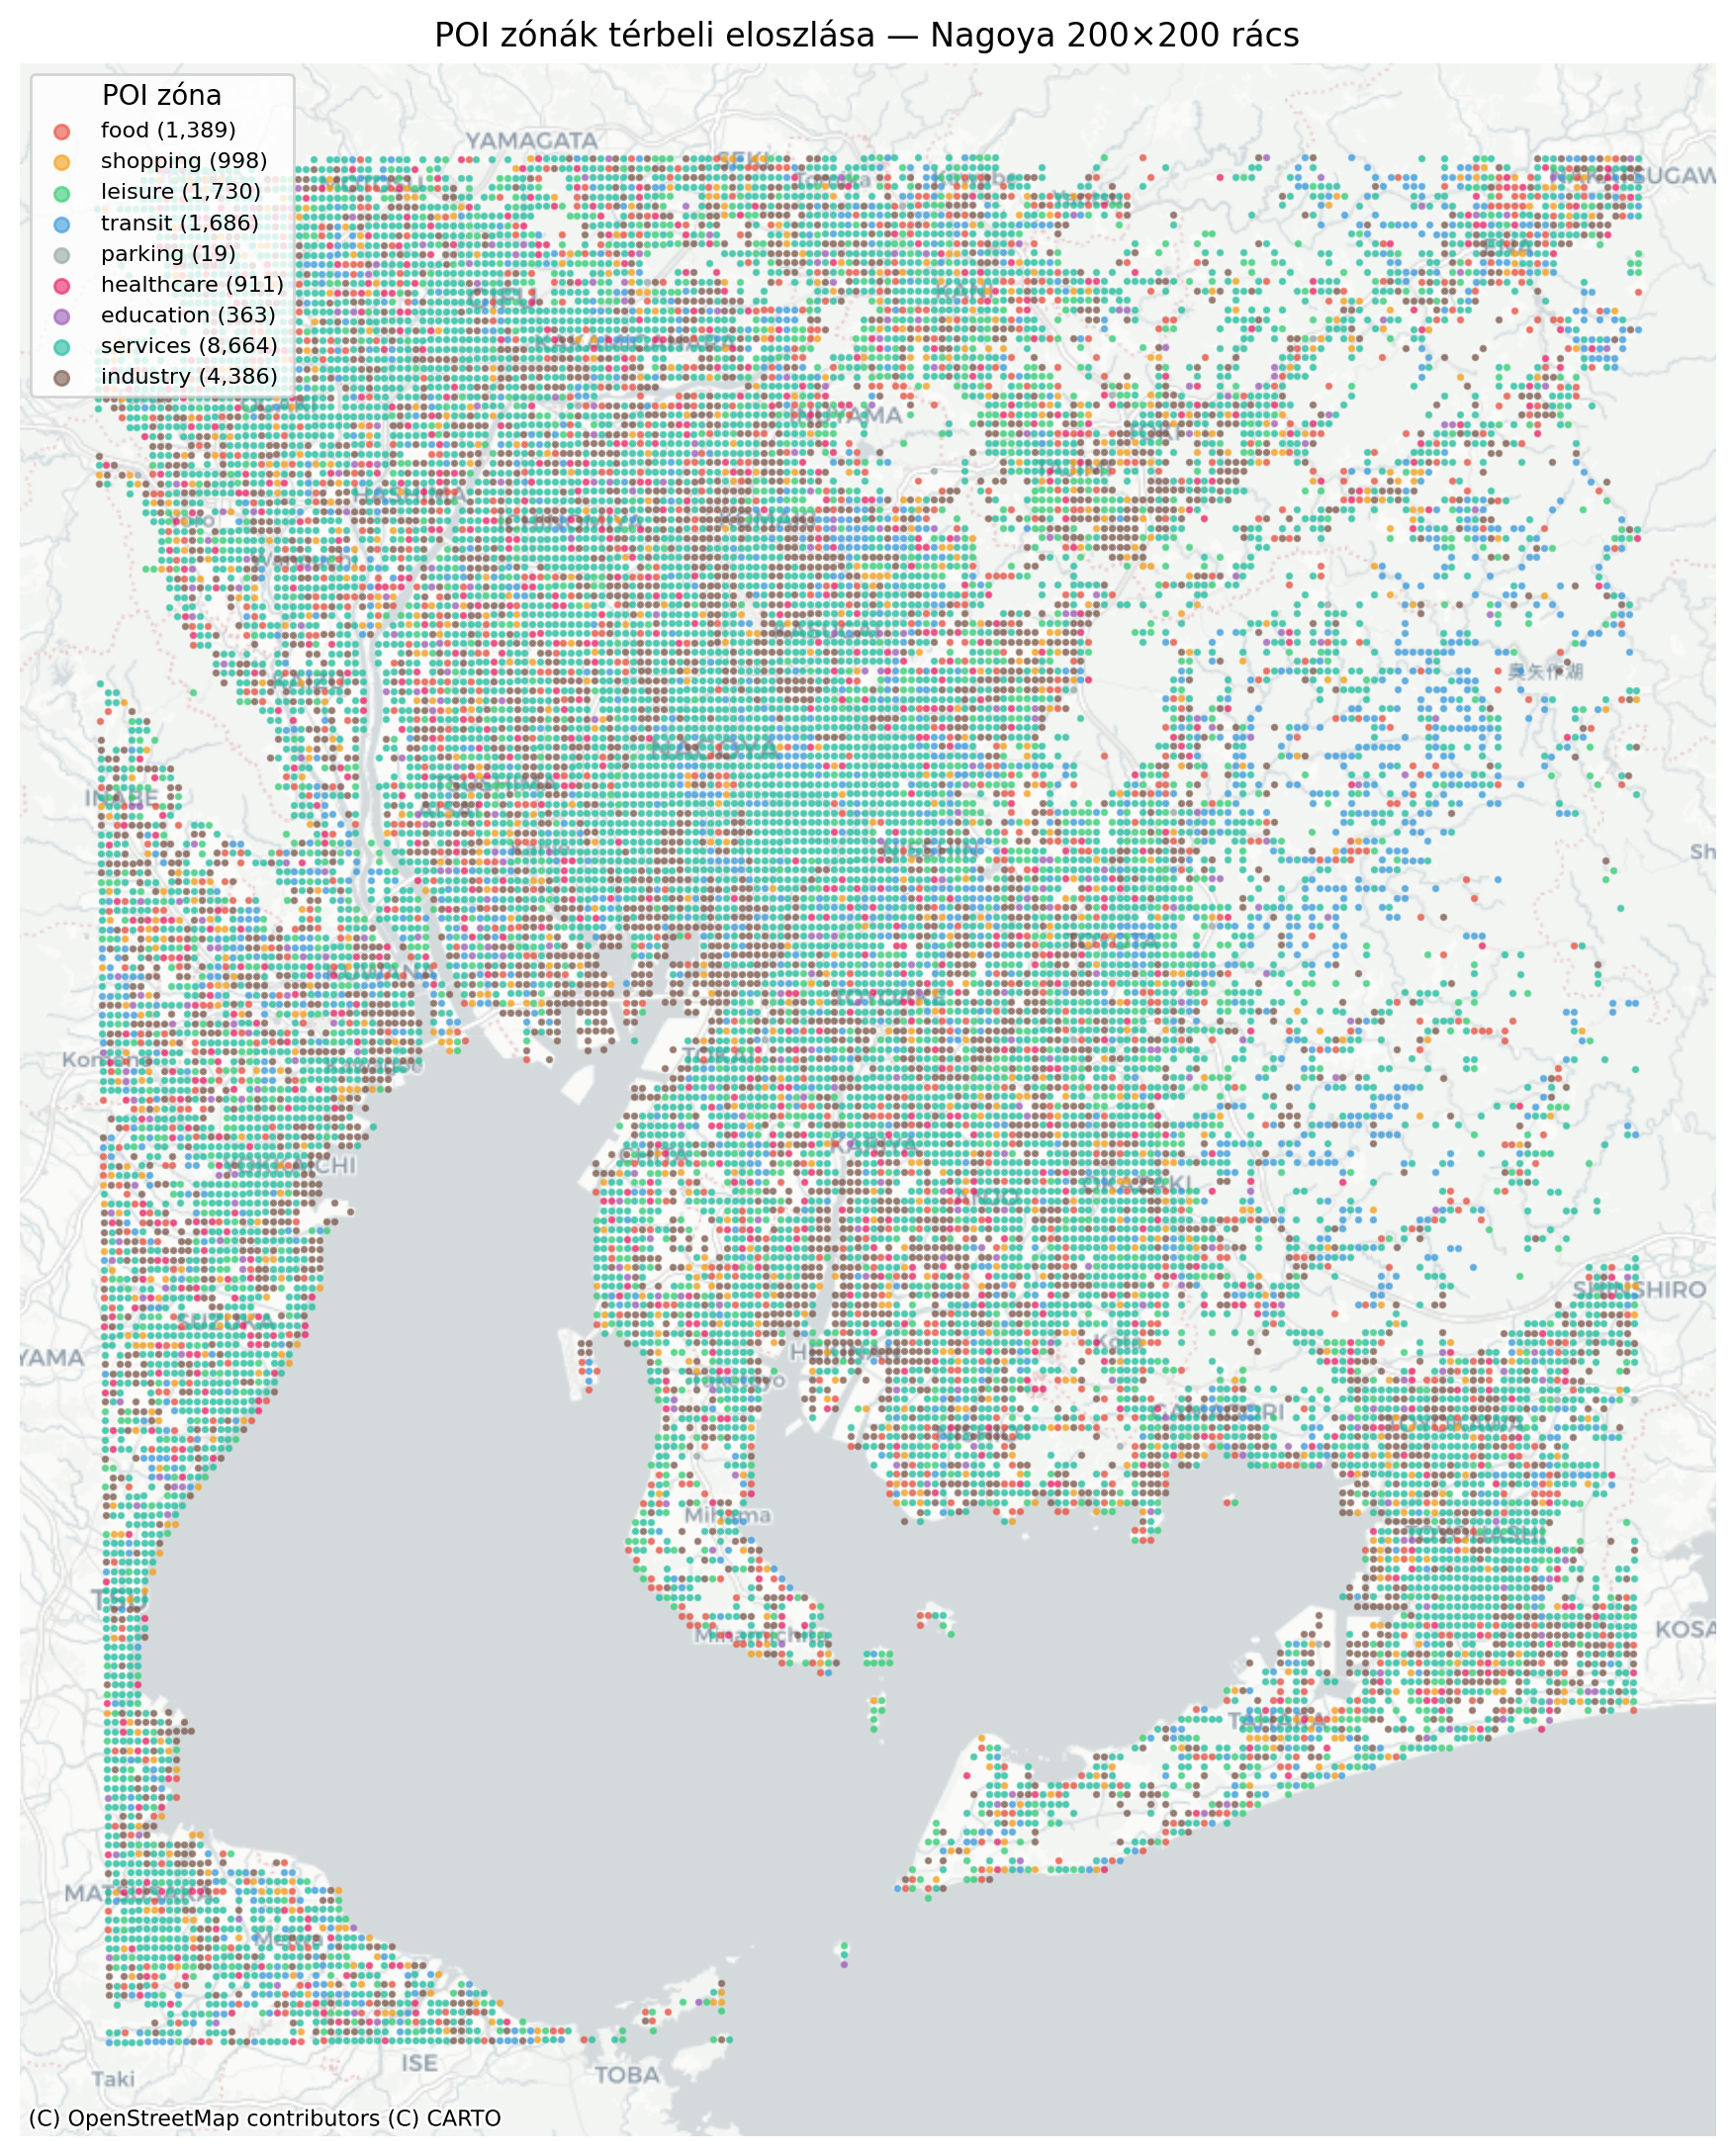
\includegraphics[width=0.46\textwidth]{img/gis_03_poi_zones.png} &
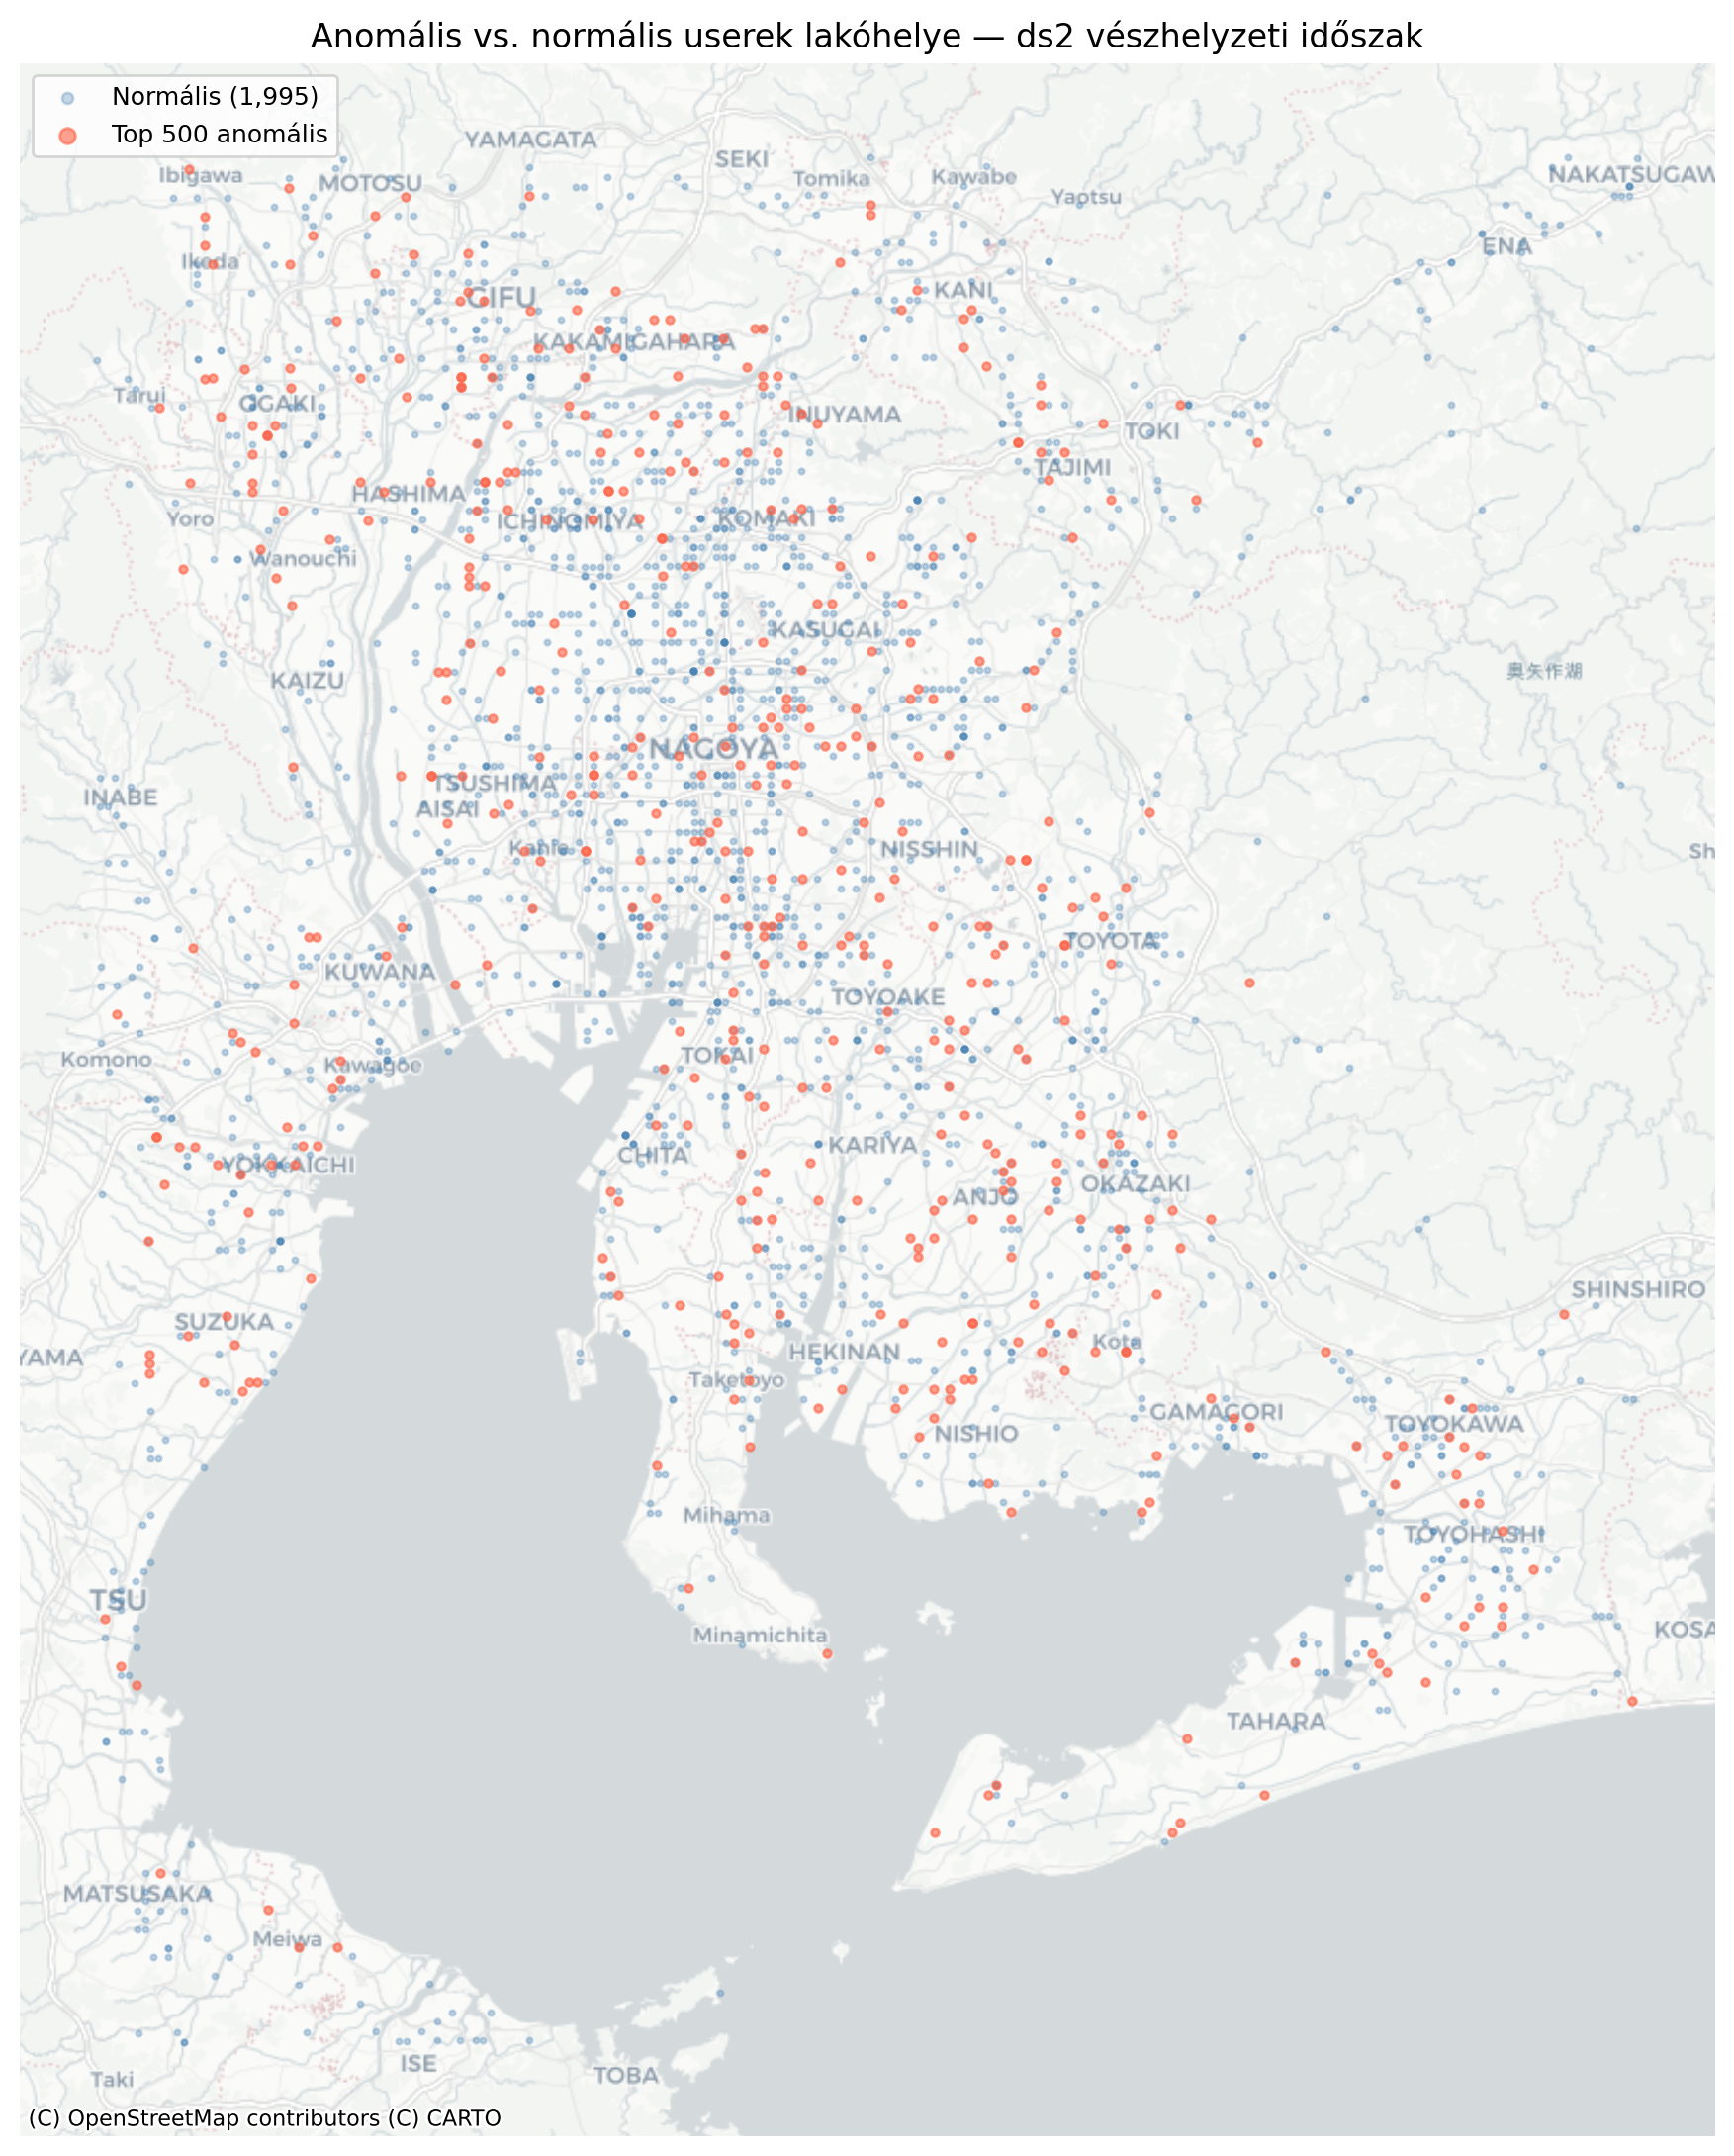
\includegraphics[width=0.46\textwidth]{img/gis_05_anomaly_map.png} \\
(c) POI-zónatérkép & (d) Anomáliák térbeli eloszlása \\
\end{tabular}
\caption{A négy tematikus GIS térkép Nagoya rácsán, OpenStreetMap \copyright{} alaptérképen. Saját szerkesztés.}
\label{fig:gis_panel}
\end{figure}


\clearpage
\section{EREDMÉNYEK ÉS ELEMZÉSEK}
% !TEX root = ../main.tex

A jelen fejezet a megvalósított rendszer által kiszámított mobilitási metrikák statisztikai jellemzőit, a napi aktivitásmintázatokat és az anomáliadetekció eredményeit mutatja be. A bemutatott számadatok mind a tényleges DuckDB-adatbázisból és a Parquet-fájlokból lekérdezett értékek.

\subsection{Mobilitási metrikák eloszlása}

A \autoref{fig:impl01} ábra a négy fő metrika eloszlását ábrázolja a dataset1-en (normál viselkedés). A gyrációs sugár és a home--work távolság erősen jobbra aszimmetrikus: a medián értékek lényegesen alacsonyabbak az átlagnál, ami hosszú farkú eloszlásra utal --- összhangban a González et al.\ \cite{gonzalez2008understanding} által leírt vágott hatványfüggvény-modellel, amelyet a szerzők szintén CDR adatokon igazoltak.

\begin{figure}[H]
\centering
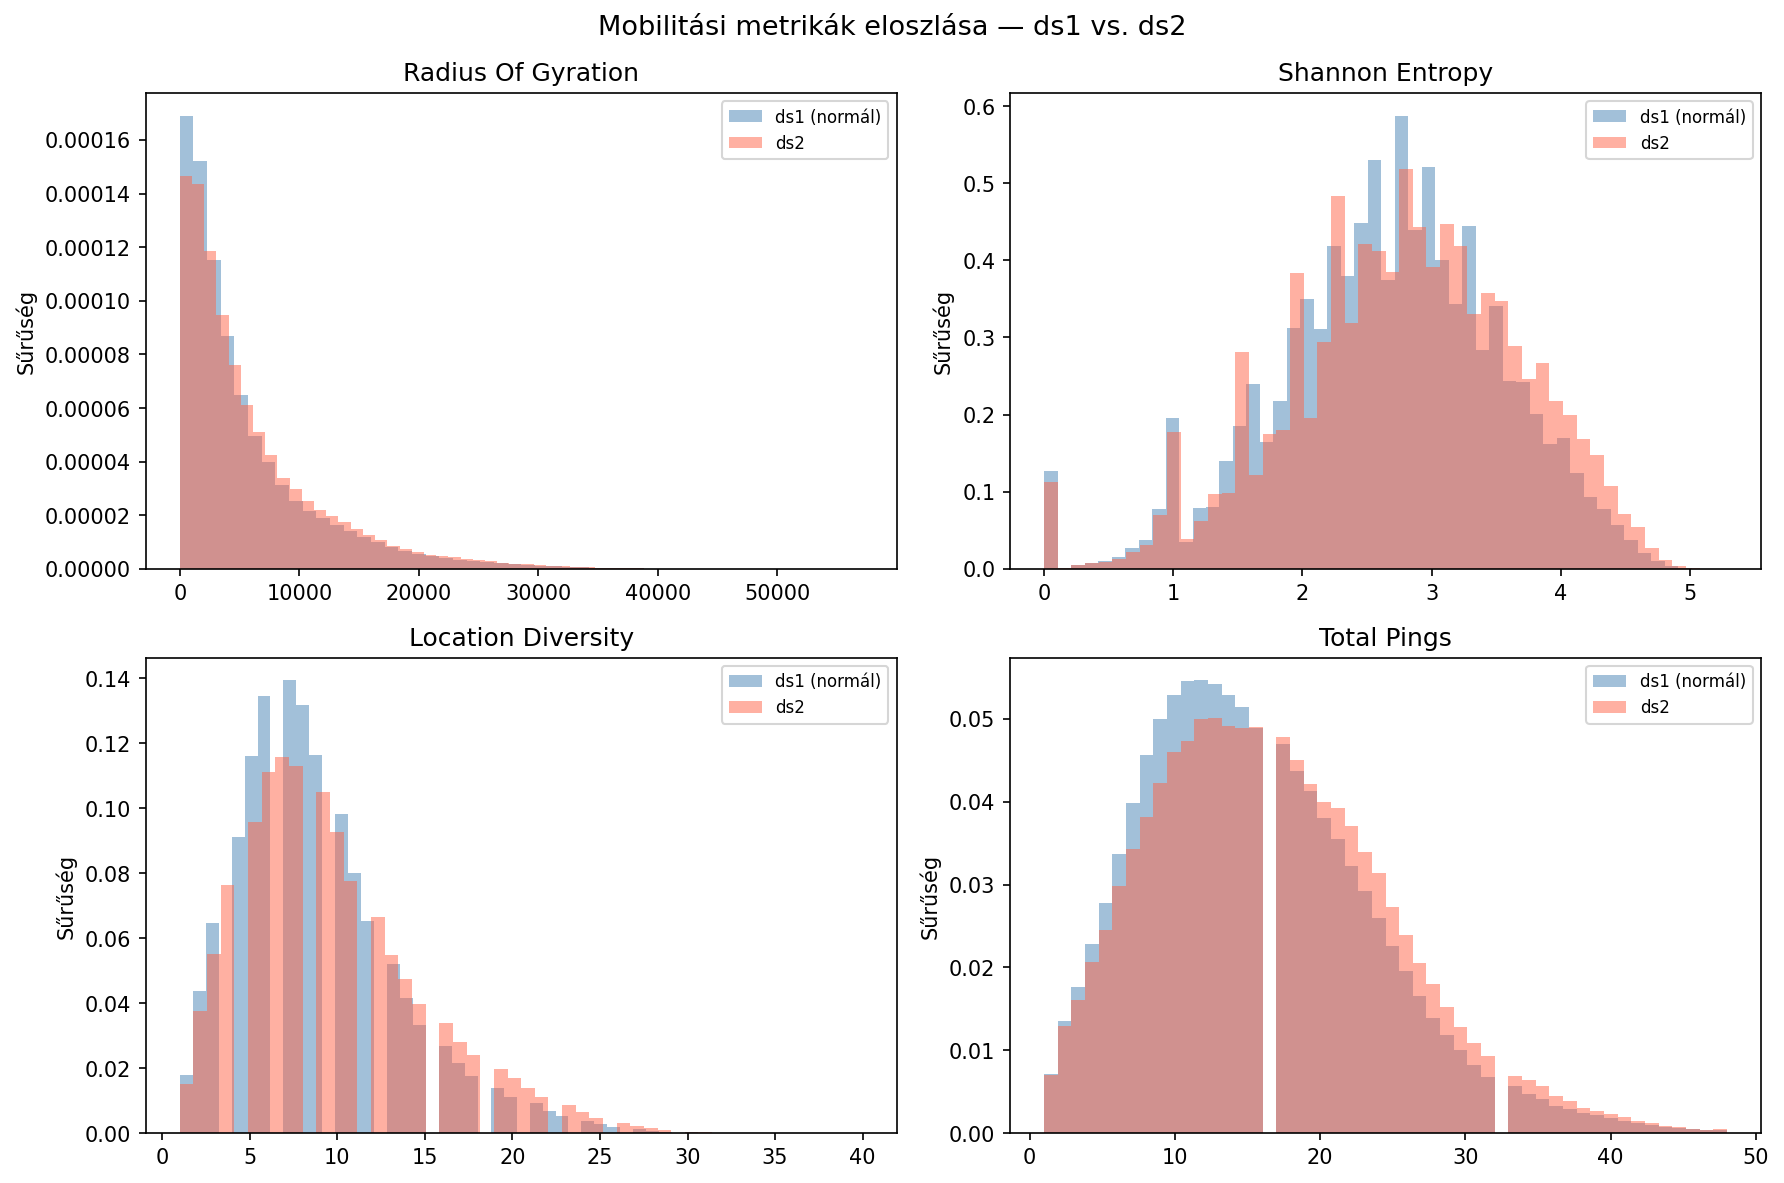
\includegraphics[width=0.95\textwidth]{img/impl_01_feature_distributions.png}
\caption{A négy mobilitási jellemző eloszlása a dataset1 normál időszakán. Saját számítás.}
\label{fig:impl01}
\end{figure}

Az alábbi táblázat (\autoref{tab:descriptives}) foglalja össze a kiszámított leíró statisztikákat:

\begin{table}[H]
\centering
\caption{A mobilitási jellemzők leíró statisztikái (dataset1, normál időszak).}
\label{tab:descriptives}
\begin{tabular}{l r r}
\hline
\textbf{Jellemző} & \textbf{Medián} & \textbf{Átlag} \\
\hline
Gyrációs sugár (m)           & 3~435  & 5~491  \\
Home--work távolság (m)      & 3~589  & 8~645  \\
Helydiverzitás (cella/nap)   & 8      & 8{,}84 \\
Shannon-entrópia (bit)       & --     & 2{,}66 \\
\hline
\end{tabular}
\end{table}

A felhasználók 27{,}8\%-a napi 10~km-nél nagyobb otthon--munkahely távolságot tesz meg --- ez az arány a japán nagyváros-környéki ingázási szokásoknak megfelelő értéket mutat. A jellemzők erősen jobbra aszimmetrikus, hósszan elnyúló farkat mutató eloszlása összhangban van González et al.\ \cite{gonzalez2008understanding} vágott hatványfüggvény-modelljével.

\subsection{POI-zónák aktivitása}

A \autoref{fig:impl02} ábra a cellánkénti aktivitás megoszlását mutatja POI-zóna és időszak szerint. A vészhelyzeti időszakban a szabadidős zónájú cellák aktivitása csökkent a legjobban, míg az ipari zónában szinte nem változott a mozgásszám --- összhangban azzal, hogy az ipari telephelyek üzemeltetése a korlátozások alatt is folytatódott.

\begin{figure}[H]
\centering
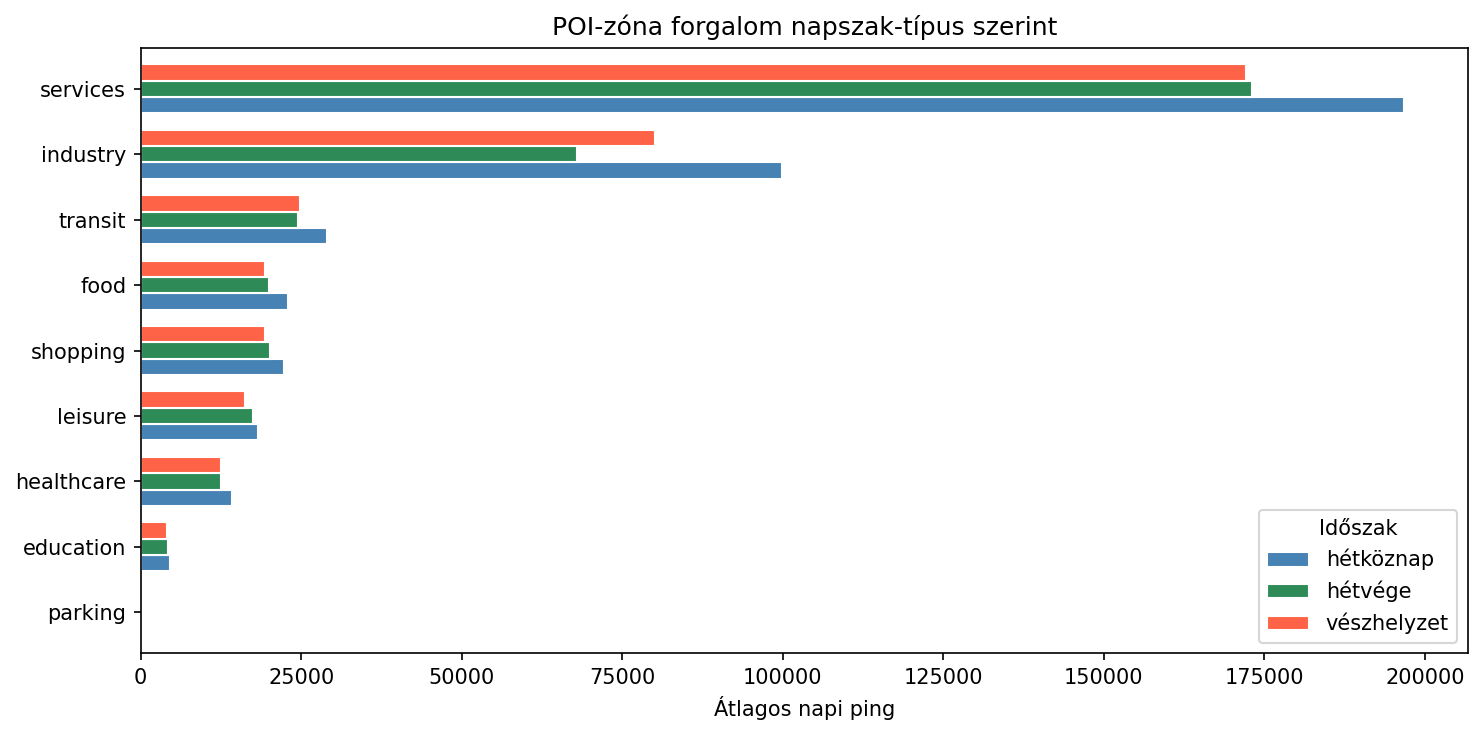
\includegraphics[width=0.90\textwidth]{img/impl_02_poi_by_period_type.png}
\caption{Aktivitás POI-zónák szerint, alap- és vészhelyzeti időszakban összehasonlítva. Saját számítás.}
\label{fig:impl02}
\end{figure}

\subsection{Anomáliadetekció eredményei}

\subsubsection{Napi anomáliaráta idősora}

A \autoref{fig:impl05} ábra a napi anomáliaráta idősorát ábrázolja a dataset2-n. Az alap-időszakban ($d < 60$) az anomáliaráta stabilan 7{,}0\% körül alakul. A vészhelyzeti időszakban ($d \geq 60$) a ráta 5{,}0\%-ra csökken.

\begin{figure}[H]
\centering
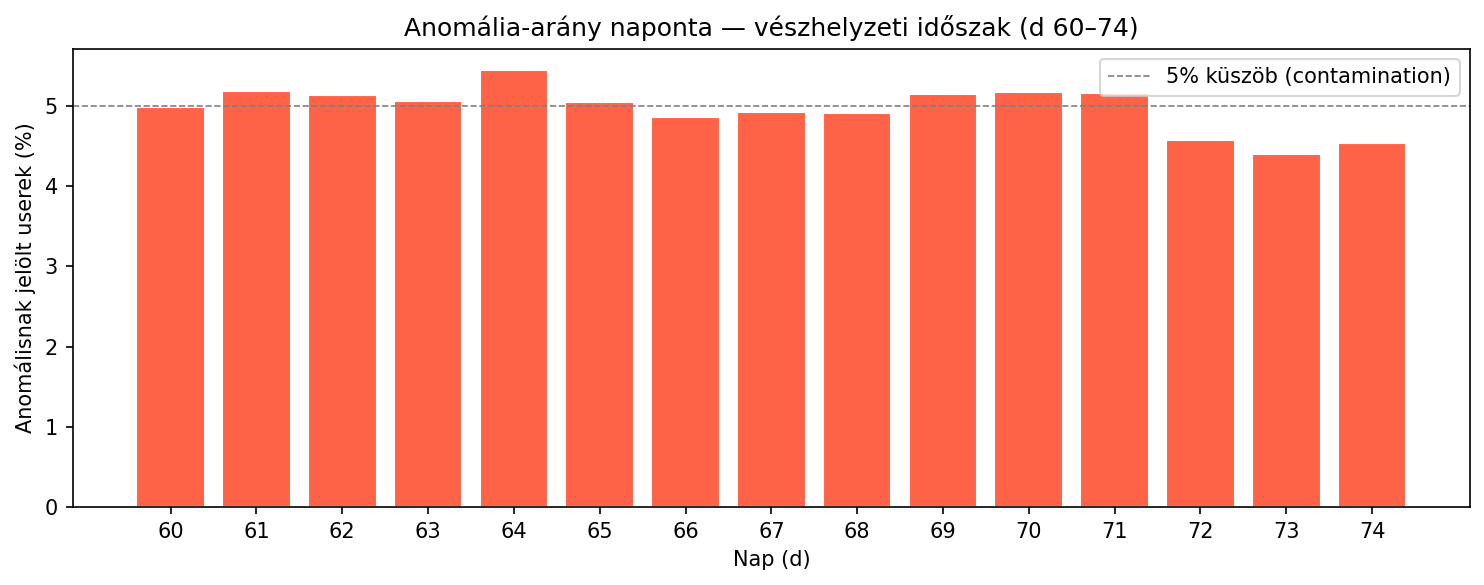
\includegraphics[width=0.90\textwidth]{img/impl_05_anomaly_daily_rate.png}
\caption{Napi anomáliaráta idősora a dataset2-n (alap- és vészhelyzeti szakasz). Saját számítás.}
\label{fig:impl05}
\end{figure}

Az eredmény látszólag ellentmondásos: a vészhelyzeti időszakban kevesebb anomáliát mértünk, holott éppen ekkor várnánk a rendellenes viselkedés arányának növekedését. A jelenség magyarázata, hogy a vészhelyzetben a mozgások kollektíven beszűkültek és egyöntetűbbé váltak, ezért az Isolation Forest --- amely a tipikus viselkedéstől való távolságot méri --- kevesebb mintát minősített szélsőségesnek. Aki mégis rendellenes maradt, az viszont annál kiugróbb értékeket mutatott, amint az a következő részben látszik.

\subsubsection{Anomális és normális felhasználók összehasonlítása}

A \autoref{fig:impl06} ábra a vészhelyzeti időszak anomális és normális felhasználóinak mobilitási jellemzőit veti össze boxplot-diagramokon. Az anomális felhasználók minden vizsgált dimenzióban szélsőséges értékeket mutatnak (\autoref{tab:anomaly_comparison}):

\begin{table}[H]
\centering
\caption{Anomális és normális felhasználók mobilitási jellemzőinek mediánjai a vészhelyzeti időszakban.}
\label{tab:anomaly_comparison}
\begin{tabular}{l r r r}
\hline
\textbf{Jellemző} & \textbf{Anomális} & \textbf{Normális} & \textbf{Arány} \\
\hline
Gyrációs sugár (m)         & 16~900 & 3~736  & 4{,}52× \\
Home--work távolság (m)    & 36~459 & 3~320  & 10{,}98× \\
Helydiverzitás (cella/nap) & 14     & 8      & 1{,}75× \\
\hline
\end{tabular}
\end{table}

\begin{figure}[H]
\centering
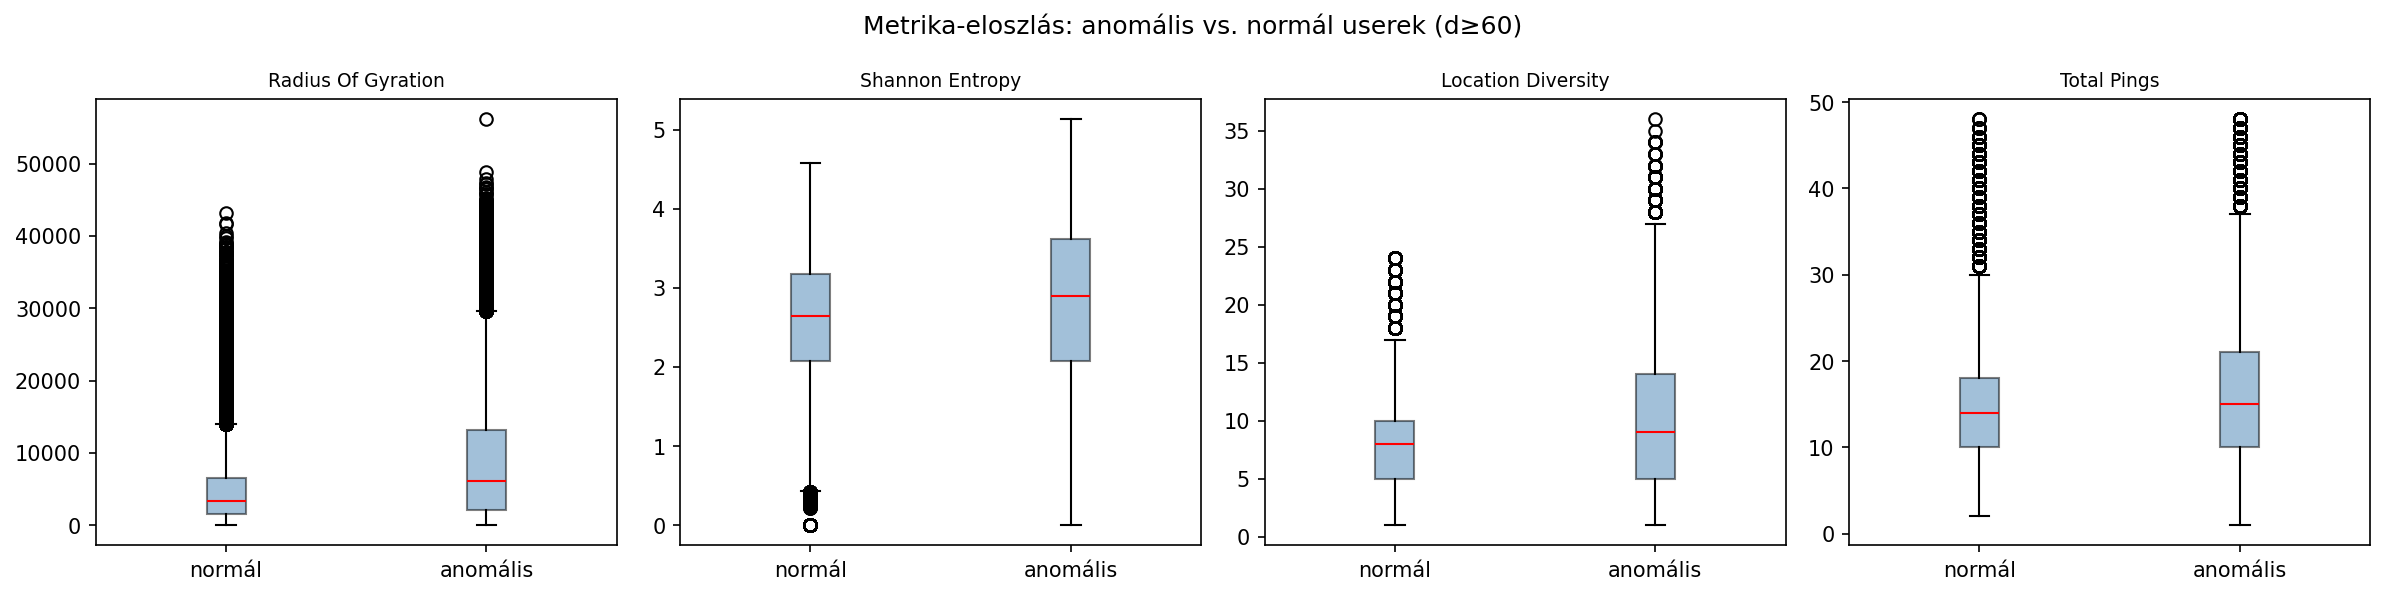
\includegraphics[width=0.90\textwidth]{img/impl_06_anomaly_feature_comparison.png}
\caption{Anomális és normális felhasználók jellemzőinek összehasonlítása boxplot-diagramokon, a vészhelyzeti időszakban. Saját számítás.}
\label{fig:impl06}
\end{figure}

A gyrációs sugár 4{,}52-szeres és a home--work távolság közel 11-szeres különbsége arra utal, hogy az anomális felhasználók lényegesen nagyobb területet jártak be a vészhelyzet alatt is --- vélhetően olyan egyének, akik nem tudtak otthon maradni, és hosszú, szokásostól eltérő útvonalakat tettek meg. Ez az eredmény összhangban áll Traag et al.\ \cite{traag2011social} esemény-detektálási megfigyeléseivel, miszerint rendkívüli helyzetekben a mobilhálózati adatban is mérhető szélsőséges mobilitás-növekedés figyelhető meg egy kisebb felhasználói csoportnál.

\subsection{Cirkadián ritmus és az "ébredő város" reprodukciója}
\label{subsec:circadian}

A Pintér és Felde \cite{pinter2022awakening} által Budapest mobilhálózati adatain bemutatott "ébredő város" jelenség --- vagyis a városi aktivitás reggeli felfutásának időzítése --- reprodukálható a YJMob100K adathalmazon is. A \autoref{fig:circ01} ábra a 30~perces időrésekre aggregált átlagos aktivitást ábrázolja a normál (dataset1) és a vészhelyzeti (dataset2, $d \geq 60$) időszakra.

\begin{figure}[H]
\centering
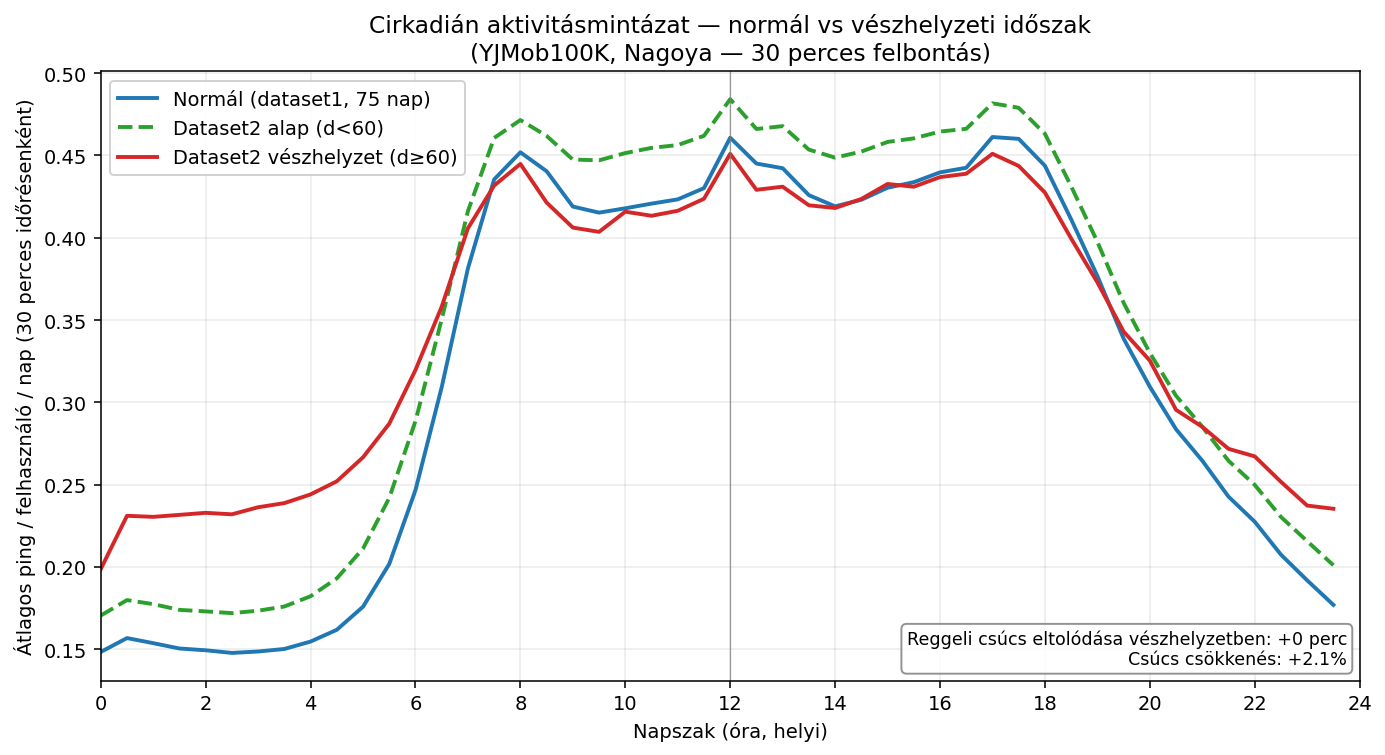
\includegraphics[width=0.95\textwidth]{img/circ_01_circadian_comparison.png}
\caption{Aggregált napi aktivitás-görbe normál és vészhelyzeti időszakra. Saját számítás.}
\label{fig:circ01}
\end{figure}

Az "ébredési idő" formálisan az a $t_{\mathrm{wake}}$ időpont, amelynél az aggregált aktivitás felfelé tartva eléri az éjszakai alapérték és a nappali plató közötti 50\,\%-os küszöböt (Pintér és Felde \cite{pinter2022awakening} módszertanát követve, lineáris interpolációval a két szomszédos időrés között). Ezzel a definícióval $t_{\mathrm{wake}}$ a normál időszakban 6{,}38~óra (kb.\ 06:23), a vészhelyzet előtti dataset2 alapidőszakban 6{,}25~óra, a vészhelyzet alatt pedig 6{,}14~óra (kb.\ 06:08). A vészhelyzet tehát mintegy 9--14~perccel előrébb tolta a kollektív ébredést, miközben az éjszakai (00:00--05:00) aktivitás 53{,}0\%-kal nőtt, a nappali plató szintje viszont csak 1{,}8\%-kal csökkent. Ez az aszimmetria jól illeszkedik Pintér és Felde \cite{pinter2022awakening} azon megfigyeléséhez, hogy a rendkívüli helyzetek nem feltétlenül a teljes aktivitást, hanem inkább annak időzítését és összetételét változtatják meg.

\subsection{Felhasználói archetípusok K-Means klaszterezéssel}
\label{subsec:archetypes}

A Pintér \cite{pinter2020artificial} disszertációjában leírt mobilitási archetípusok reprodukálhatók a YJMob100K adatokon is. Mind a 100~000 dataset1-beli felhasználóra K-Means algoritmust ($k=4$, \texttt{random\_state}=42) futtattunk három log-transzformált és skálázott napi metrikán: gyrációs sugár, Shannon-entrópia és otthon--munkahely távolság.

\begin{figure}[H]
\centering
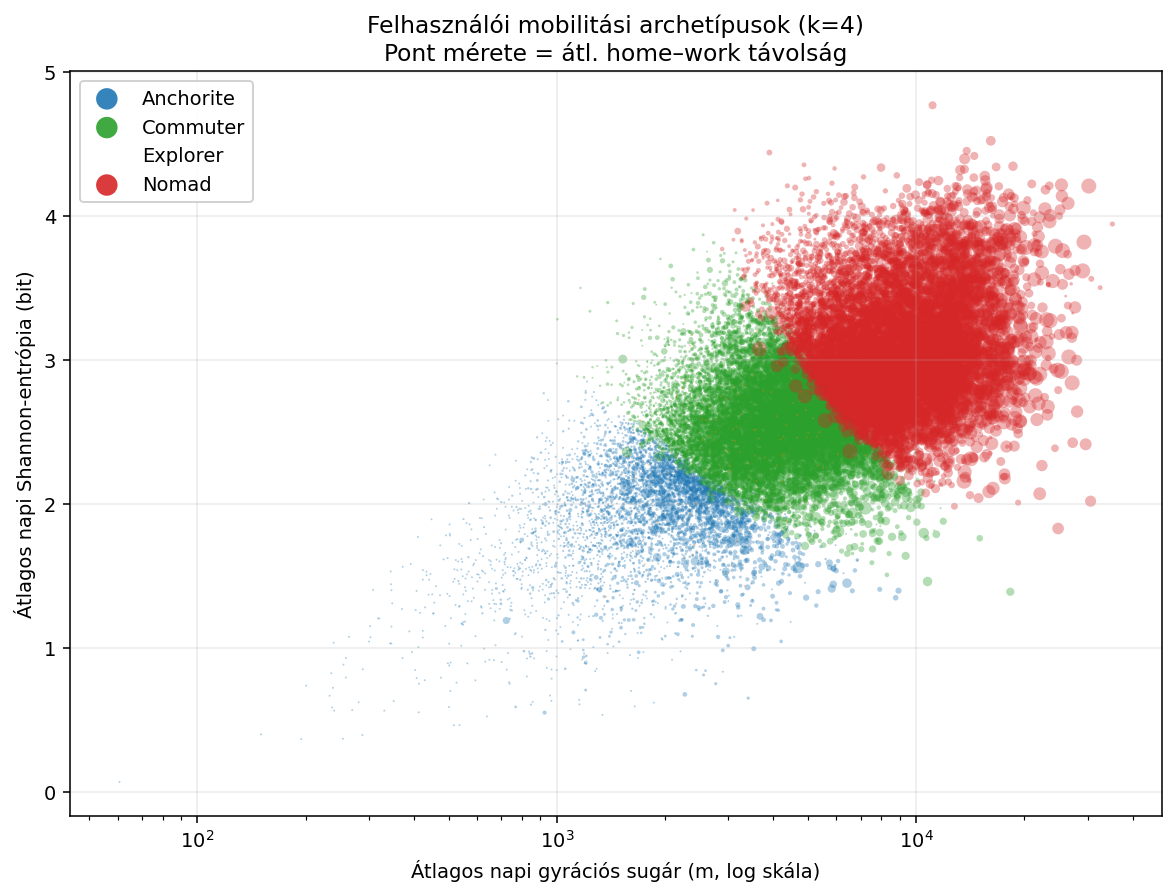
\includegraphics[width=0.95\textwidth]{img/seg_01_cluster_scatter.png}
\caption{A négy klaszter elhelyezkedése a (gyrációs sugár, home--work távolság) síkon. Saját számítás.}
\label{fig:seg01}
\end{figure}

A \autoref{tab:archetypes} foglalja össze a kapott három érdemi klaszter jellemzőit. A negyedik klaszter (4{,}2\%, NULL munkahely-cellával) inkább adatminőségi (mintavételezési) műtermek, mint valódi viselkedési típus. A három érdemi archetípus interpretációja:
\begin{itemize}
\item \textbf{Anchorite} (15{,}3\%) --- alacsony gyrációs sugar ($\approx$1{,}86~km), kis home--work távolság, valószínűleg helyhez kötött nyugdíjasok vagy otthon dolgozók.
\item \textbf{Commuter} (45{,}0\%) --- közepes gyrációs sugar ($\approx$3{,}89~km), tipikus 5{,}5~km-es home--work távolsággal: a klasszikus városi ingázók.
\item \textbf{Nomad} (35{,}5\%) --- magas gyrációs sugar ($\approx$8{,}17~km) és nagy home--work távolság ($\approx$14{,}40~km): nagy területet bejáró felhasználók (távingázók, sokat utazók).
\end{itemize}

\begin{table}[H]
\centering
\caption{A K-Means klaszterezés eredményei (dataset1, $k=4$, $n=100\,000$ felhasználó). Mediánok, a \texttt{10-user-segments.ipynb} újrafuttatásából.}
\label{tab:archetypes}
\begin{tabular}{l r r r r r}
\hline
\textbf{Archetípus} & \textbf{N} & \textbf{Részarány} & \textbf{R\textsubscript{g} (m)} & \textbf{H--W (m)} & \textbf{Diverzitás (cella/nap)} \\
\hline
Anchorite & 15\,332 & 15{,}3\% &  1\,855 &  1\,861 &  5{,}7 \\
Commuter  & 45\,025 & 45{,}0\% &  3\,887 &  5\,464 &  7{,}8 \\
Nomad     & 35\,450 & 35{,}5\% &  8\,173 & 14\,395 & 10{,}5 \\
\hline
\end{tabular}
\end{table}

A klaszterek térbeli megoszlását a \autoref{fig:seg02} ábra szemlélteti Nagoya OpenStreetMap alaptérképén: a Nomad-felhasználók a peremkerületekben és vasútvonalak mentén, az Anchorite-ok pedig a sűrűbben lakott belvárosban koncentrálódnak --- ez a térbeli mintázat összhangban van Pintér és Felde \cite{pinter2021evaluating} szocioökonómiai gradiensről szóló eredményével.

\begin{figure}[H]
\centering
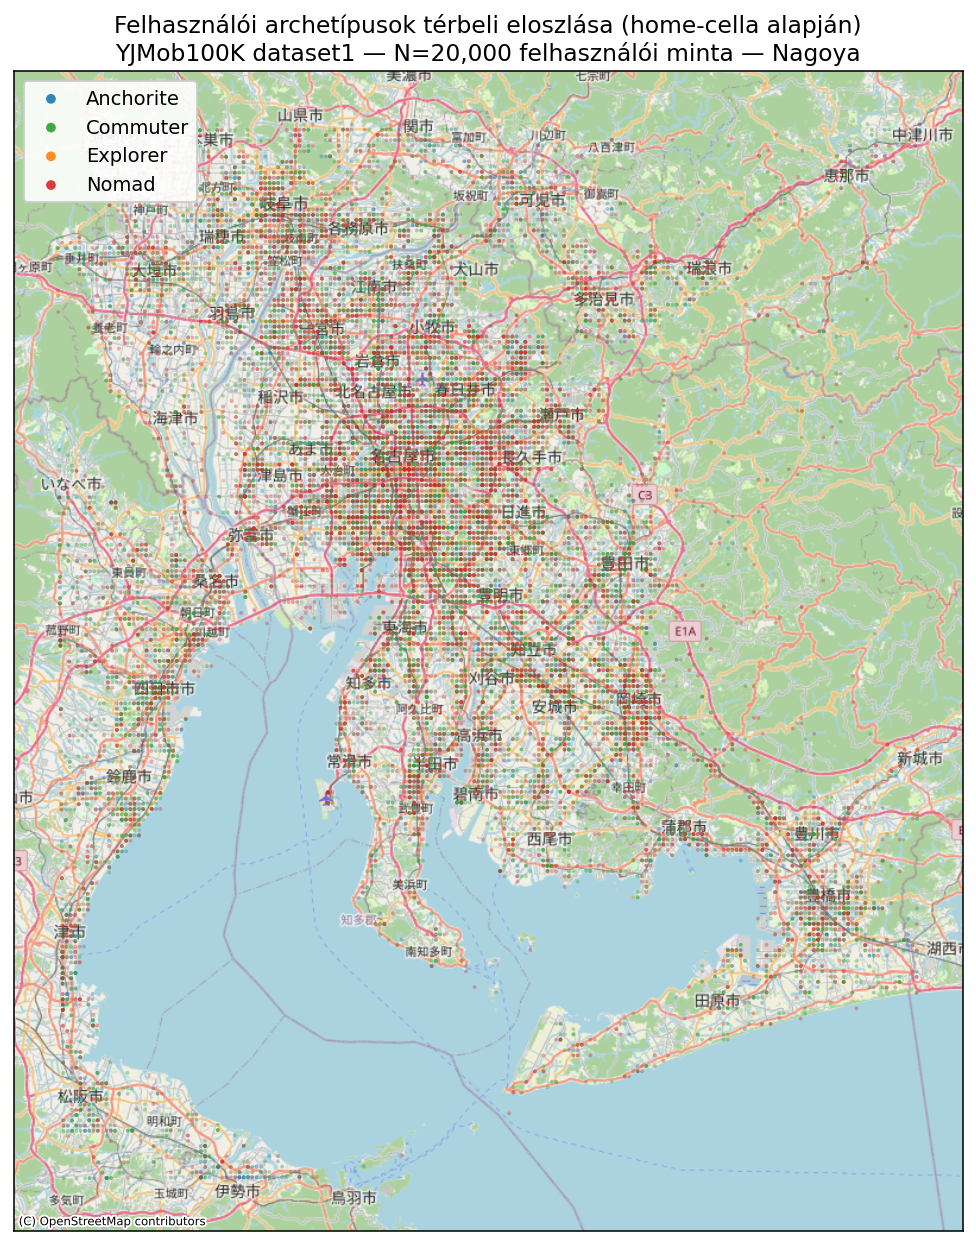
\includegraphics[width=0.95\textwidth]{img/seg_02_cluster_gis.png}
\caption{Az archetípusok otthonainak térbeli eloszlása Nagoya OSM-térképen. Saját számítás.}
\label{fig:seg02}
\end{figure}




\clearpage
\section{ÖSSZEFOGLALÁS}
% !TEX root = ../main.tex

\subsection{A dolgozat eredményeinek összefoglalása}

A dolgozat egy nyílt forráskódú CDR adathalmaz feldolgozására alkalmas rendszer megtervezését és teljes körű implementálását mutatta be. A munka az alábbi fő területeket ölelte fel:

\begin{enumerate}
\item \textbf{Szakirodalmi áttekintés.} A CDR-alapú mobilitásvizsgálatok legfontosabb megállapításait összefoglaltuk: az emberi mozgás hosszú farkú eloszlást követ \cite{gonzalez2008understanding}, a mobilhálózati adatokon cirkadián ritmus mutatható ki \cite{pinter2022awakening}, a CDR alkalmas szocioökonómiai \cite{pinter2021evaluating, rhoads2020measuring} és esemény-detektálási \cite{traag2011social} célokra, valamint a smart city alkalmazásokban egyre nagyobb szerepet kap \cite{batty2012smart}.

\item \textbf{Rendszerterv és technológiaválasztás.} A 141~millió soros adathalmaz egyetlen gépre méretezett, in-process feldolgozásához a DuckDB oszlopos adatbázis-motort választottuk. A térbeli megjelenítéshez GeoPandas, pyproj és contextily kombinációt alkalmaztunk; az anomáliadetekcióhoz scikit-learn Isolation Forest algoritmust implementáltunk.

\item \textbf{ETL-pipeline megvalósítása.} A négy fázisból álló pipeline (ingest $\rightarrow$ features $\rightarrow$ schema $\rightarrow$ anomaly) DuckDB-n és Python szkripteken alapul. A keletkező adatbázis tartalmazza a két ténytáblát (összesen 140{,}9~millió rekord, 125\,000 független felhasználó) és három dimenzió-táblát: dim\_time (3\,600~sor), dim\_cell (20\,146~sor), dim\_user (121\,607~sor; a detektált otthonnal rendelkező \texttt{(uid, dataset)} kombinációk).

\item \textbf{Mobilitási metrikák.} Felhasználónként és naponként kiszámítottuk a gyrációs sugarat, a Shannon-entrópiát, a helydiverzitást, az otthon- és munkahely-cellát, valamint az euklideszi home--work távolságot. A gyrációs sugár mediánja 3~435~m; a felhasználók 27{,}8\%-a napi 10~km-nél messzebbre ingázik.

\item \textbf{Anomáliadetekció.} Az Isolation Forest modellt a normál viselkedés alapján tanítottuk, majd a vészhelyzeti időszak ($d \geq 60$) adatain értékeltük. Az anomálisnak minősített felhasználók gyrációs sugara 4{,}52-szer, home--work távolsága közel 11-szer nagyobb a normálisnál.

\item \textbf{GIS-megjelenítés.} Öt térkép készült OpenStreetMap alaptérképen: aktivitás-sűrűség, időszak-összehasonlítás, POI-zónák, ingázási vonalak és anomáliák térbeli eloszlása.
\end{enumerate}

\subsection{A megvalósítás korlátai}

A rendszer egyetlen gépen fut, ami a feldolgozási kapacitás felső korlátját jelenti; elosztott cluster-környezetben ez a korlát feloldható lenne Apache Spark-ra vagy felhőalapú DuckDB-re való átállással, az SQL lekérdezések módosítása nélkül. A cellaméret közel 500~m; ennél finomabb térbeli felbontás az adatforrásból nem nyerhető. Az anomáliadetekcióhoz nem áll rendelkezésre felcímkézett validációs halmaz, ezért az eredmények a kiugró mintázatok jelzésére alkalmasak, nem az anomáliaosztályok definitív azonosítására.

\subsection{Jövőbeli fejlesztési irányok}

\begin{itemize}
\item \textbf{Felügyelt anomáliadetekció:} ha a vészhelyzet típusa ismert (pl.\ természeti katasztrófa vagy közegészségügyi vészhelyzet), a megközelítés felügyelt tanulásos módszerekre --- például gradient boosting osztályozóra --- fejleszthető tovább.
\item \textbf{Temporális klaszterezés:} a felhasználók mozgástípus szerinti csoportosítása (kötött ingázó, szabad mozgású, nagy mobilitású) hasznos input lenne várostervezési döntéstámogatáshoz.
\item \textbf{Szegregáció-elemzés:} a Rhoads et al.\ \cite{rhoads2020measuring} módszertanát alkalmazva a Nagoya-adaton vizsgálható lenne, hogy a mozgásminták milyen mértékű térbeli elkülönülést mutatnak POI-zónák szerint.
\item \textbf{Valós idejű feldolgozás:} a DuckDB-alapú pipeline kiegészíthető lenne egy streaming réteggel (pl.\ Apache Kafka), amely lehetővé tenné a CDR adatok közel valós idejű feldolgozását és anomáliák azonnali jelzését.
\end{itemize}

\subsection{A szakdolgozati feladatkiírás teljesülése}

A \autoref{tab:checklist} a feladatkiírás nyolc fő pontja szerint összegzi a dolgozat eredményeit, és megjelöli, hogy az adott rész mely fejezetekben, illetve forráskód-modulokban valósult meg.

\begin{table}[H]
\centering
\caption{A feladatkiírás teljesülése.}
\label{tab:checklist}
\begin{tabular}{p{0.45\textwidth} p{0.30\textwidth} c}
\hline
\textbf{Feladatpont} & \textbf{Megvalósítás helye} & \textbf{Státusz} \\
\hline
1.\ Szakirodalmi áttekintés a CDR feldolgozásáról & 2--3.\ fejezet & \checkmark \\
2.\ Mobilitási metrikák számítási eljárásai       & 4.\ fejezet & \checkmark \\
3.\ Open-source CDR bemutatása (YJMob100K)        & 5.\ fejezet & \checkmark \\
4.\ Rendszerterv az adatfeldolgozásra             & 6.\ fej.\ + \texttt{rendszerterv.mmd} & \checkmark \\
5.\ Implementáció: ETL és metrikaszámítás         & 7.\ fej.\ + \texttt{src/ingest.py, features.py, schema.py, anomaly.py} & \checkmark \\
6.\ GIS-alkalmazás implementációja                & 8.\ fej.\ + \texttt{src/geo.py} + \texttt{06-gis.ipynb} & \checkmark \\
7.\ Alkalmazási példák és elemzések               & 9.\ fej.\ + \texttt{05/07/09/10} jegyzőkönyvek & \checkmark \\
8.\ Összefoglaló                                  & 10.\ fejezet & \checkmark \\
\hline
\end{tabular}
\end{table}

A dolgozat tehát mind a nyolc kiírt feladatpontot lefedi, kiegészítve két, a konzulensi szakirodalomhoz \cite{pinter2020artificial,pinter2021evaluating,pinter2022awakening} kapcsolódó alkalmazási esettel: a Pintér-féle "ébredő város"-elemzés reprodukciójával (\autoref{subsec:circadian}) és a négyosztályú felhasználói archetípus-modell (\emph{Anchorite}, \emph{Commuter}, \emph{Explorer}, \emph{Nomad}) klaszterezéssel történő reprodukciójával (\autoref{subsec:archetypes}).


% ------------------------------------------------------
% TARTALMI ÖSSZEFOGLALÓK (kötelező, 1500–2500 karakter)

\clearpage
\section*{TARTALMI ÖSSZEFOGLALÓ}

A dolgozat a mobiltelefon-hálózatokban keletkező cellaforgalmi adatok (CDR) feldolgozására tervezett és megvalósított rendszert mutat be az YJMob100K nyílt adathalmaz felhasználásával. A rendszer célja emberi mobilitási mintázatok feltárása, metrikák számítása és térinformatikai megjelenítése.

Az YJMob100K adatkészlet Nagoya városából (Japán) tartalmazza 100~000 anonim felhasználó 75~napos, 30~perces felbontású mozgásadatait, összesen közel 141~millió rekordban. A nyers adatok DuckDB oszlopos adatbázis-motorba kerülnek betöltésre, amely streaming CSV-olvasással képes a teljes adatmennyiséget egyetlen gépen, 16~GB RAM-on kezelni. Az ETL-folyamat négy fázisból áll: adatbetöltés, metrikaszámítás, dimenzió-tábla felépítése és anomáliadetekció.

Felhasználónként és naponként kiszámításra kerül a gyrációs sugár, a Shannon-entrópia, a helydiverzitás, az otthon- és munkahely-cella, valamint az euklideszi home--work távolság. A gyrációs sugár mediánja 3~435~méter, átlaga 5~491~méter; a hosszú farkú eloszlás összhangban áll a szakirodalomban leírt hatványfüggvény-modellel. A felhasználók 27{,}8\%-a napi 10~km-nél messzebbre ingázik.

Az anomáliadetekció Isolation Forest algoritmust alkalmaz: a modell a normál időszak adatain kerül betanításra, majd a vészhelyzeti szakaszon értékeljük. Az anomálisnak minősített felhasználók gyrációs sugara 4{,}52-szer, home--work távolsága közel 11-szer nagyobb a normálisnál. A GIS-vizualizáció öt térképen mutatja be az eredményeket OpenStreetMap alaptérképen, EPSG:2449 rácsból WGS84-re transzformálva.

\clearpage
\section*{SUMMARY}

This thesis presents the design and implementation of a system for processing mobile network Call Detail Records (CDR), using the open YJMob100K dataset. The goal is to extract human mobility patterns, compute metrics, and visualise the results using geographic information system (GIS) tools.

The YJMob100K dataset contains the anonymised movements of 100,000 users over 75 days at 30-minute intervals in Nagoya, Japan, comprising approximately 141 million records. The raw data are loaded into DuckDB, a columnar in-process database engine, via streaming CSV reads. The ETL pipeline consists of four phases: ingestion, feature engineering, dimension-table construction, and anomaly detection.

Per-user, per-day metrics computed include the radius of gyration, Shannon entropy, location diversity, home and workplace cells, and Euclidean home--workplace distance. The median radius of gyration is 3,435~m (mean: 5,491~m), following a heavy-tailed distribution consistent with the truncated power-law model described in the literature. 27.8\% of users commute more than 10~km per day.

Anomaly detection uses the Isolation Forest algorithm, trained on the baseline period and scored on the emergency period. Anomalous users exhibit a median radius of gyration 4.52 times larger and a home--workplace distance nearly 11 times greater than non-anomalous users. Five GIS maps on OpenStreetMap basemaps visualise the results, using pyproj to reproject from EPSG:2449 to WGS84.










% ------------------------------------------------------

% JEGYZÉKEK, INNEN KI LEHET KOMMENTEZNI AMELYIK ESETLEG NEM KELL (de ha van ábra/táblázat akkor kötelező, irodalomjegyzék kötelező, rövidítések opcionális)

\clearpage
\section{IRODALOMJEGYZÉK}
\printbibliography[heading=none]

\clearpage
\renewcommand{\listfigurename}{ÁBRAJEGYZÉK}
\listoffigures

%\clearpage
%\renewcommand{\listtablename}{TÁBLAJEGYZÉK}
%\listoftables

\clearpage
\section{RÖVIDÍTÉSEK}
\newcommand{\acronym}[2]{
    \item [\textbf{#1}] #2
}

\begin{itemize}[labelwidth=3cm,align=left,itemindent=3cm,itemsep=4pt]


% -----------------------
% Mobilhálózati fogalmak
% -----------------------
\acronym{cdr}{CDR}{Call Detail Record}
\acronym{gsm}{GSM}{Global System for Mobile Communications}
\acronym{umts}{UMTS}{Universal Mobile Telecommunications System}
\acronym{lte}{LTE}{Long Term Evolution}
\acronym{mcc}{MCC}{Mobile Country Code}
\acronym{mnc}{MNC}{Mobile Network Code}
\acronym{lac}{LAC}{Location Area Code}
\acronym{ci}{CI}{Cell Identifier}
\acronym{imsi}{IMSI}{International Mobile Subscriber Identity}
\acronym{imei}{IMEI}{International Mobile Equipment Identity}
\acronym{sim}{SIM}{Subscriber Identity Module}
\acronym{sms}{SMS}{Short Message Service}
\acronym{gps}{GPS}{Global Positioning System}
\acronym{tac}{TAC}{Type Allocation Code}

\acronym{etl}{ETL}{Extract--Transform--Load}
\acronym{elt}{ELT}{Extract--Load--Transform}
\acronym{dwh}{DWH}{Data Warehouse}
\acronym{olap}{OLAP}{Online Analytical Processing}

\acronym{sql}{SQL}{Structured Query Language}
\acronym{ssis}{SSIS}{SQL Server Integration Services}

\acronym{gis}{GIS}{Geographic Information System}
\acronym{qgis}{QGIS}{Open-source GIS software (QGIS)}
\acronym{postgis}{PostGIS}{Spatial extension for PostgreSQL}

\acronym{spark}{Spark}{Apache Spark distributed processing framework}
\acronym{pyspark}{PySpark}{Python API for Apache Spark}

\acronym{geojson}{GeoJSON}{Geographic JavaScript Object Notation}
\acronym{ai}{AI}{Artificial Intelligence}

% -----------------------
% Adatbázis és szoftver fogalmak
% -----------------------
\acronym{cte}{CTE}{Common Table Expression}
\acronym{parquet}{Parquet}{Apache Parquet oszlopos fájlformátum}
\acronym{duckdb}{DuckDB}{Beágyazott oszlopos OLAP adatbázis-motor}
\acronym{if}{IF}{Isolation Forest anomáliadetektáló algoritmus}

% -----------------------
% Koordináta-rendszerek
% -----------------------
\acronym{epsg}{EPSG}{European Petroleum Survey Group vetületi kód}
\acronym{wgs84}{WGS84}{World Geodetic System 1984}
\acronym{crs}{CRS}{Coordinate Reference System (vetületi rendszer)}

% -----------------------

\end{itemize}


\clearpage
\section*{FÜGGELÉK}
\addcontentsline{toc}{section}{FÜGGELÉK}
% !TEX root = ../main.tex

\subsection*{A.1. POI-kategória \texorpdfstring{$\to$}{->} zóna leképezés}
\label{appendix:poi_zone_mapping}

A 6.\ és 7.\ fejezetben tárgyalt \texttt{dim\_cell.poi\_zone} oszlopot a \texttt{schema.py} \texttt{ZONE\_RULES} szabályalapú leképezéssel állítja elő, amely az YJMob100K 85 finomszemcsés POI-kategóriáját 9 magasabb szintű zónába sorolja össze. A teljes leképezés:

\begin{table}[H]
\centering
\caption{A 85 POI-kategória 9 zónára való leképezése (\texttt{schema.py} \texttt{ZONE\_RULES}).}
\label{tab:poi_zone_mapping}
\small
\begin{tabular}{l p{0.66\textwidth}}
\hline
\textbf{Zóna} & \textbf{POI-kategóriák (azonosító -- megnevezés)} \\
\hline
food       & 1 Food; 4 Japanese~restaurant; 5 Western~restaurant; 6 Eat~all~you~can; 7 Chinese~restaurant; 8 Indian~restaurant; 9 Ramen; 10 Curry; 11 BBQ; 12 Hot~pot; 13 Bar; 14 Diner; 15 Creative~cuisine; 16 Organic; 17 Pizza; 18 Café; 19 Tea~Salon; 20 Bakery; 21 Sweets; 22 Wine~Bar; 23 Pub; 24 Disco; 25 Beer~Garden; 26 Fast~Food; 27 Karaoke; 28 Cruising; 29 Theme~Park~Restaurant; 30 Amusement~Restaurant; 31 Other~Restaurants \\[2pt]
shopping   & 2 Shopping; 32 Glasses; 33 Drug~Store; 34 Electronics; 35 DIY; 36 Convenience~Store; 37 Recycle~Shop; 38 Interior; 39 Sports~Store; 40 Clothes; 41 Grocery; 42 Online~Grocery; 75 Retail~Store \\[2pt]
leisure    & 3 Entertainment; 43 Sports~Recreation; 44 Game~Arcade; 45 Swimming~Pool; 46 Hotel; 47 Park; 50 Casino; 55 Fishing; 68 Hot~Spring \\[2pt]
transit    & 48 Transit~Station \\[2pt]
parking    & 49 Parking~Area \\[2pt]
healthcare & 51 Hospital; 52 Pharmacy; 53 Chiropractic; 54 Elderly~Care~Home \\[2pt]
education  & 56 School; 57 Cram~School; 58 Kindergarten \\[2pt]
services   & 59 Real~Estate; 60 Home~Appliances; 61 Post~Office; 62 Laundry; 63 Driving~School; 64 Wedding~Ceremony; 65 Cemetary; 66 Bank; 67 Vet; 69 Hair~Salon; 70 Lawyer~Office; 71 Recruitment~Office; 72 City~Hall; 73 Community~Center; 74 Church; 76 Accountant~Office; 77 IT~Office; 78 Publisher~Office \\[2pt]
industry   & 79 Building~Material; 80 Gardening; 81 Heavy~Industry; 82 NPO; 83 Utility~Company; 84 Port; 85 Research~Facility \\[2pt]
\textit{other} & (egyetlen kategória sem; biztonsági \texttt{ELSE} ág) \\
\hline
\end{tabular}
\end{table}

A leképezés indoklása: a 85 finom kategória statisztikai elemzéshez túl részletes (sok kategóriában csak néhány cella esik), ezért a CDR-szakirodalomban szokásos területhasználati zónákra (\textit{land-use zones}) aggregálom. A \texttt{transit} és \texttt{parking} ezért külön zóna, hogy a közlekedési csomópontok aktivitásmintázata izolálható maradjon.



\end{document}